\indent En lo que sigue, mostraremos buenos y malos casos para nuestro algoritmo, y a su vez, daremos el tiempo estimado 
seg\'un la complejidad del algoritmo calculada anteriormente.\\


 Para obtener un mejor caso y mejorar la performance del algoritmo desarrollamos una poda o corte, la cual consiste en lo siguiente: \textbf{Cuando se encuentra el camino m\'inimo, se corta el algoritmo}.\\

Para ejemplificar lo dicho, mostraremos como se comporta el algoritmo con y sin la poda.

El mejor caso, como dijimos ser\'a el caso en que se encuentre el camino minimo m\'as r\'apido o se llegue a que no hay soluci\'on debido a la imposibilidad de romper paredes de una forma r\'apida.\\

El grafo que representa lo dicho ser\'ia el siguiente:\\

\vspace*{0.3cm} \vspace*{0.3cm}
  \begin{center}
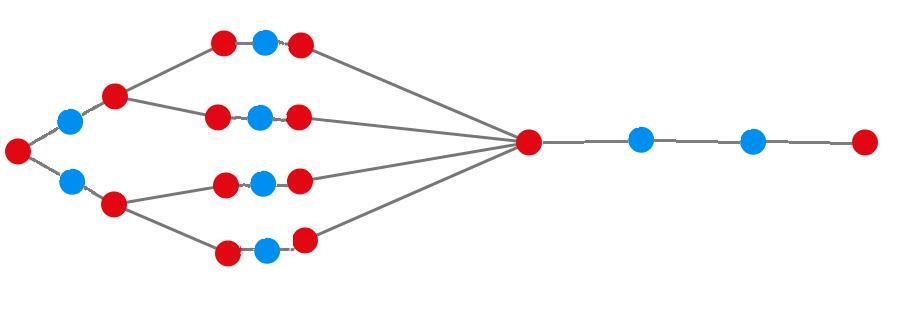
\includegraphics[scale=0.65]{./EJ1/ej1grafomejorcaso.jpeg}
{$Ejemplo Grafo$ \ G1.1 - $Mejor$ $Caso$}
  \end{center}
  \vspace*{0.3cm}


Para una mayor observaci\'on desarrollamos el siguiente gr\'afico con las instancias:\\

\vspace*{0.3cm} \vspace*{0.3cm}
  \begin{center}
 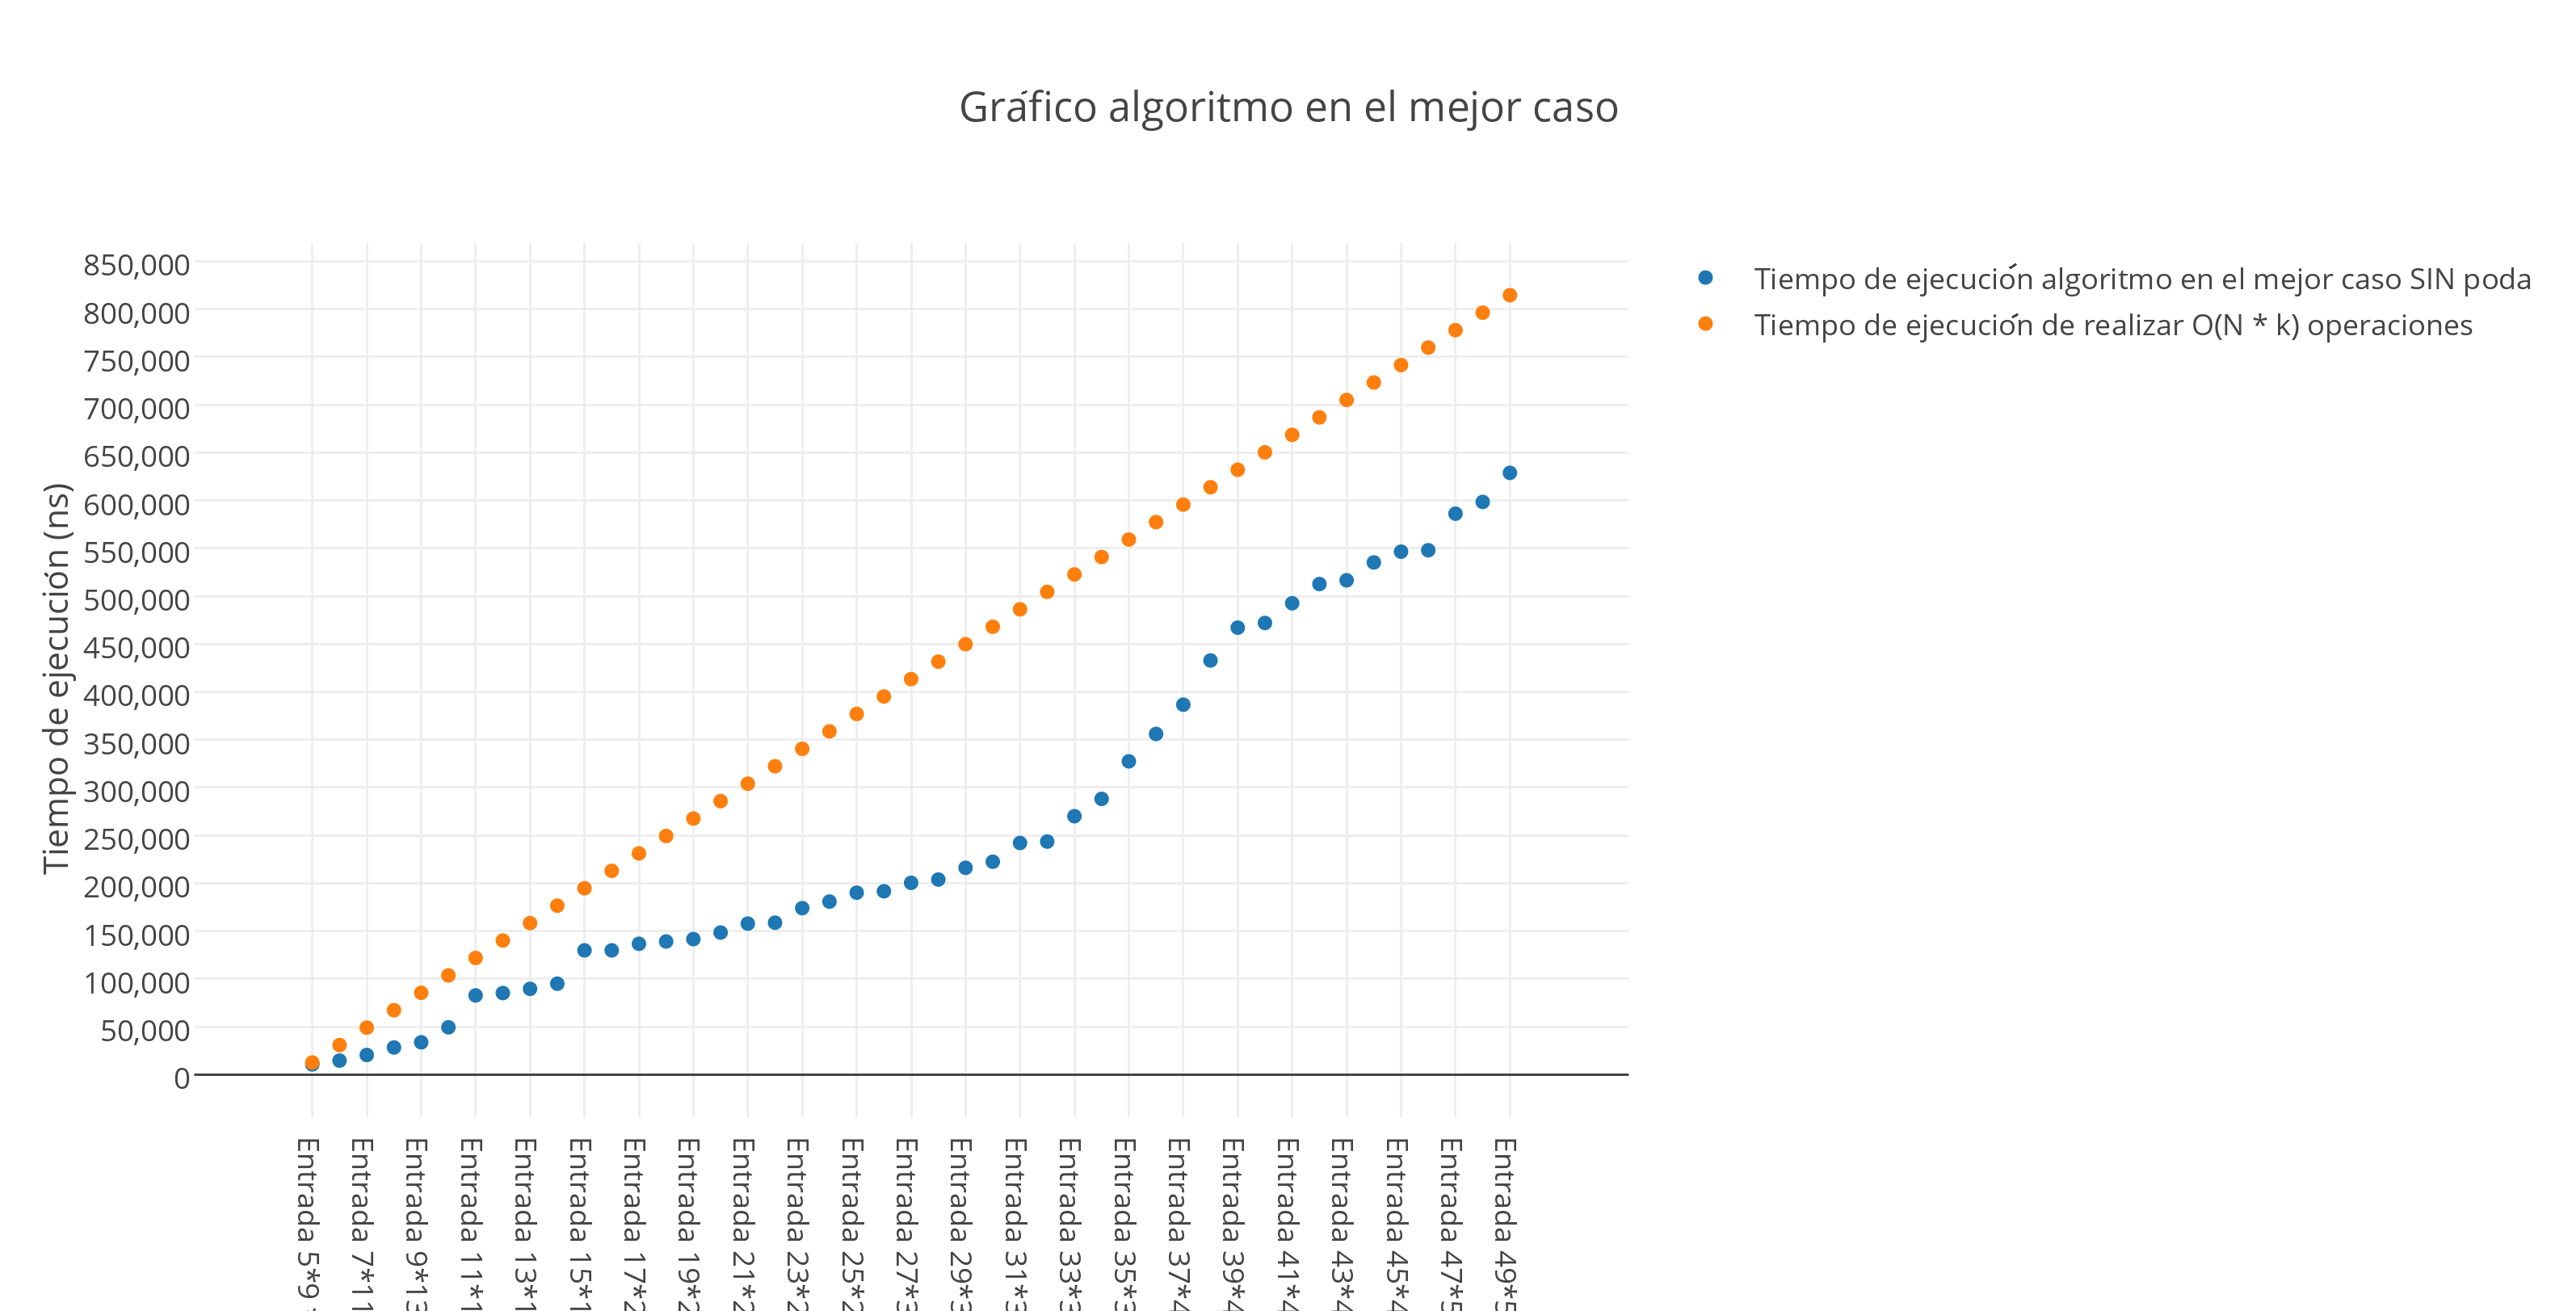
\includegraphics[scale=0.65]{./EJ1/mejorcaso.png}
 {$Gr$\'a$fico$ \ 1.1 - $Mejor$ $Caso$ $Sin$ $Poda$}
  \end{center}
  \vspace*{0.3cm}

Como la complejidad que calculamos se basa en la cantidad de nodos posibles que puede haber multiplicado por las paredes contrastaremos nuestras mediciones con los valores de N (F * C) $\ast$ P (en los gr\'aficos denominado como k).\\
A continuaci\'on mostraremos el gr\'afico comparativo de como se comporta nuestro algoritmo en el mejor caso con la poda descripta.\\

\vspace*{0.3cm} \vspace*{0.3cm}
  \begin{center}
 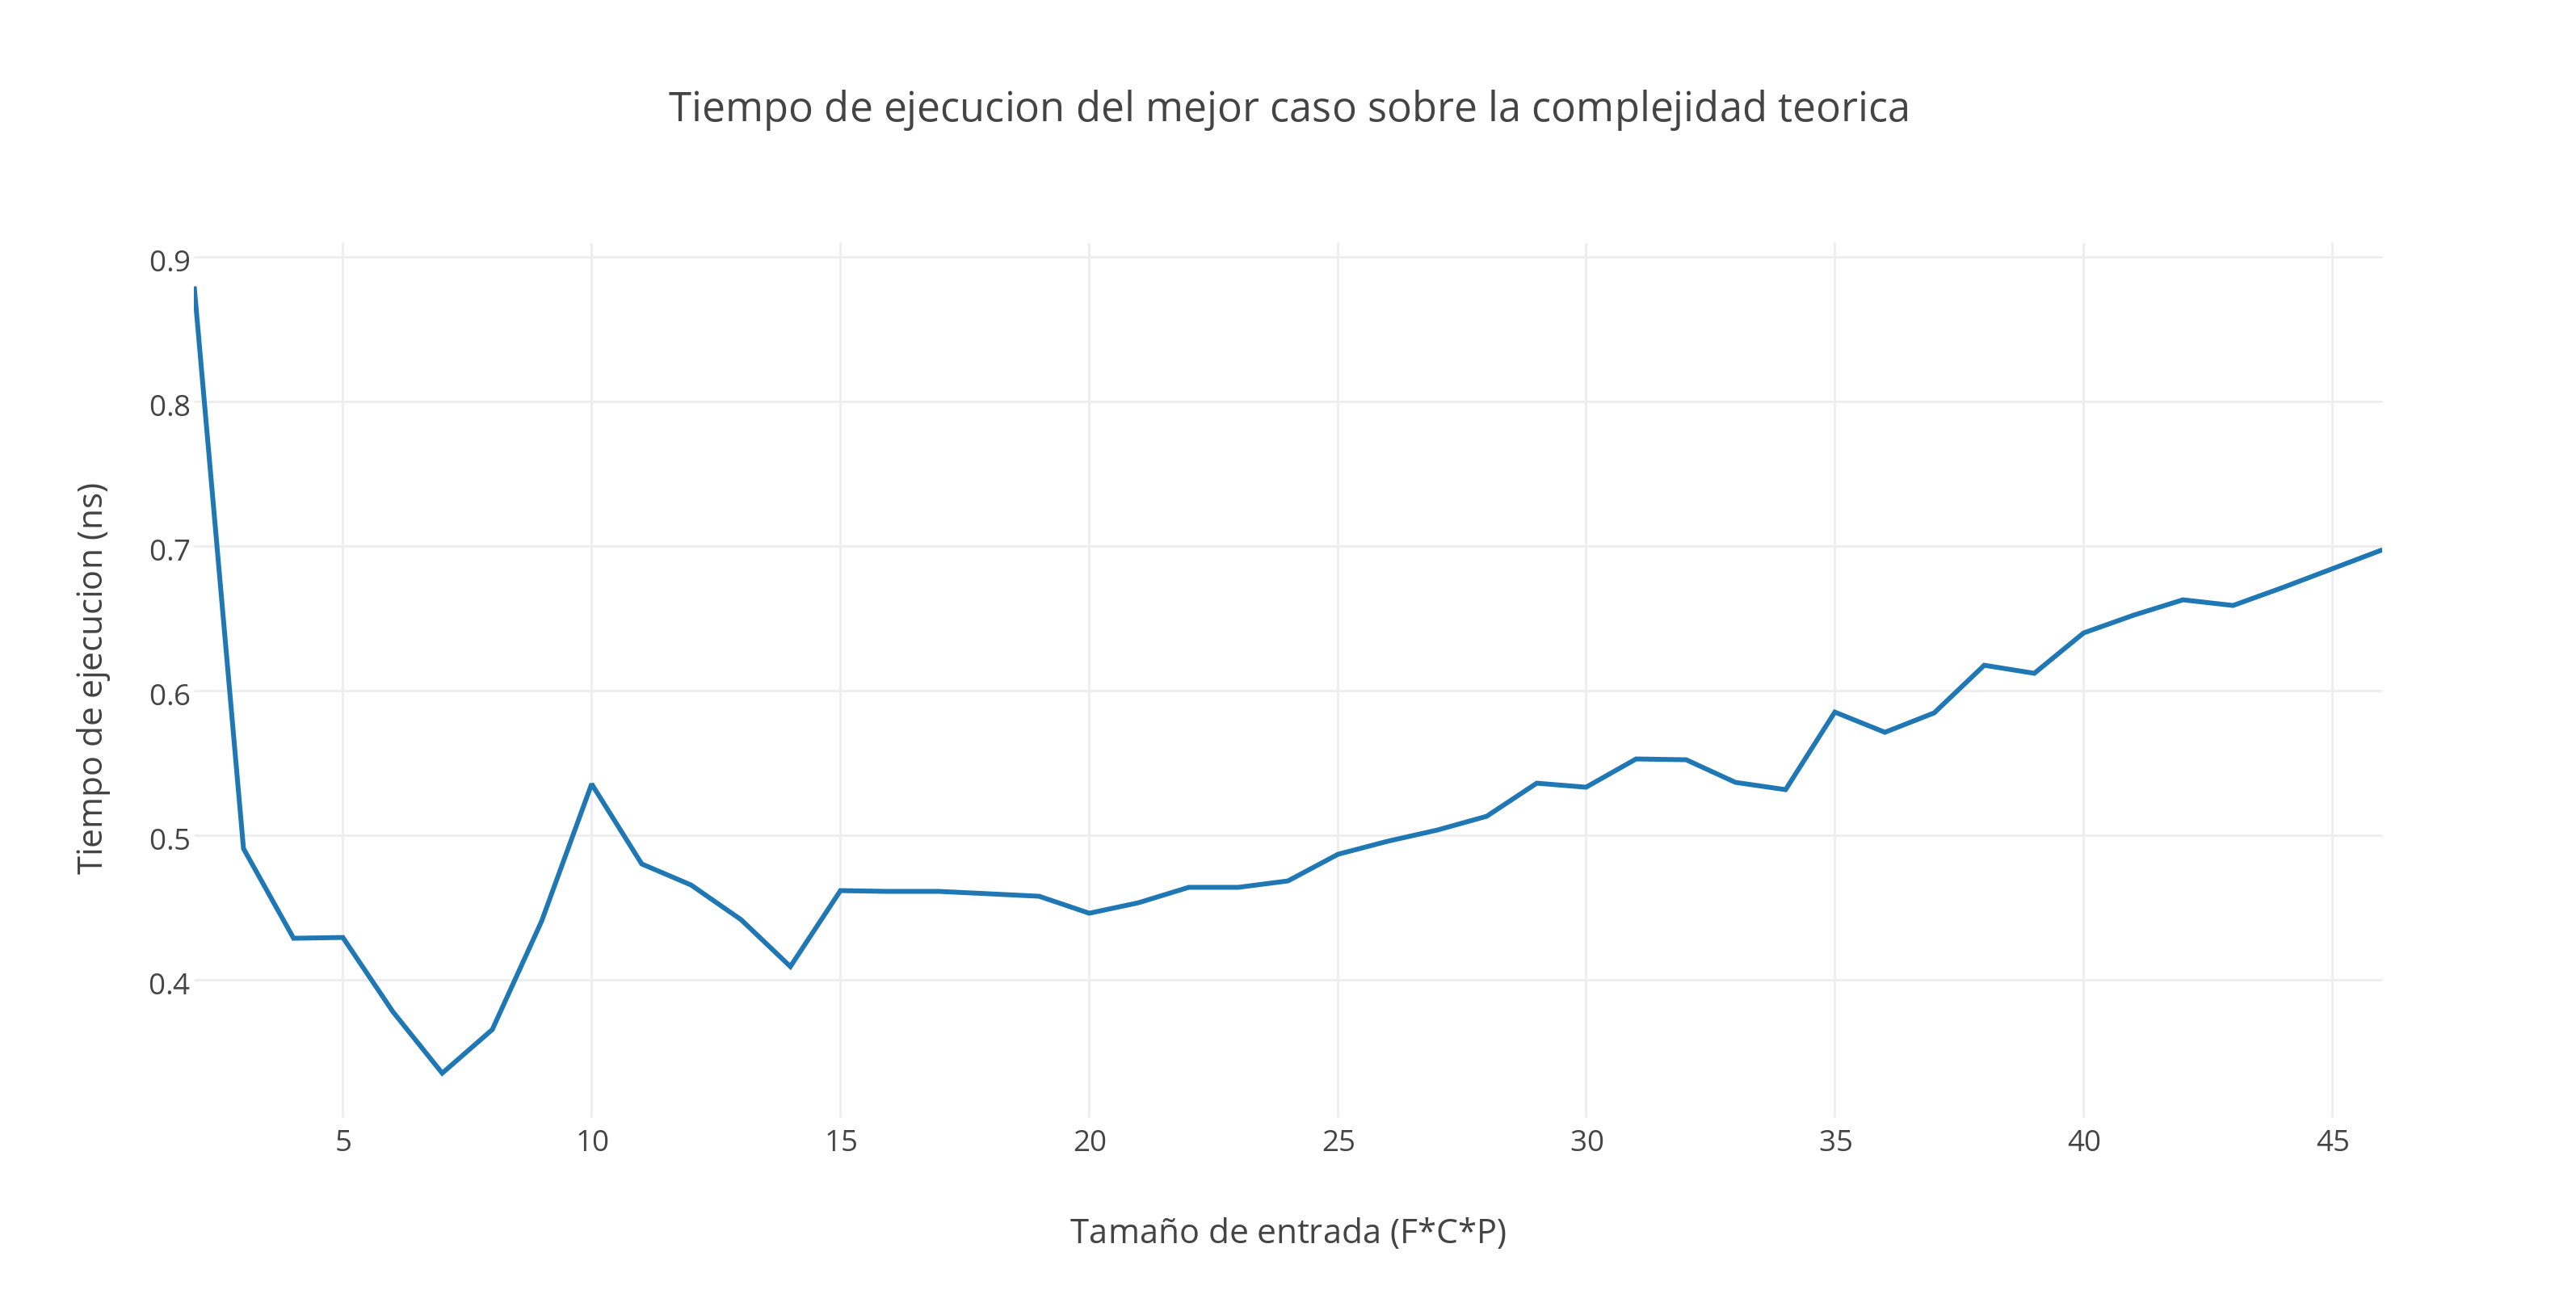
\includegraphics[scale=0.65]{./EJ1/mejorcaso1.png}
 {$Gr$\'a$fico$ \ 1.2 - $Mejor$ $Caso$ $Con$ $y$ $Sin$ $Poda$}
  \end{center}
  \vspace*{0.3cm}

\vspace*{0.3cm} \vspace*{0.3cm}
  \begin{center}
 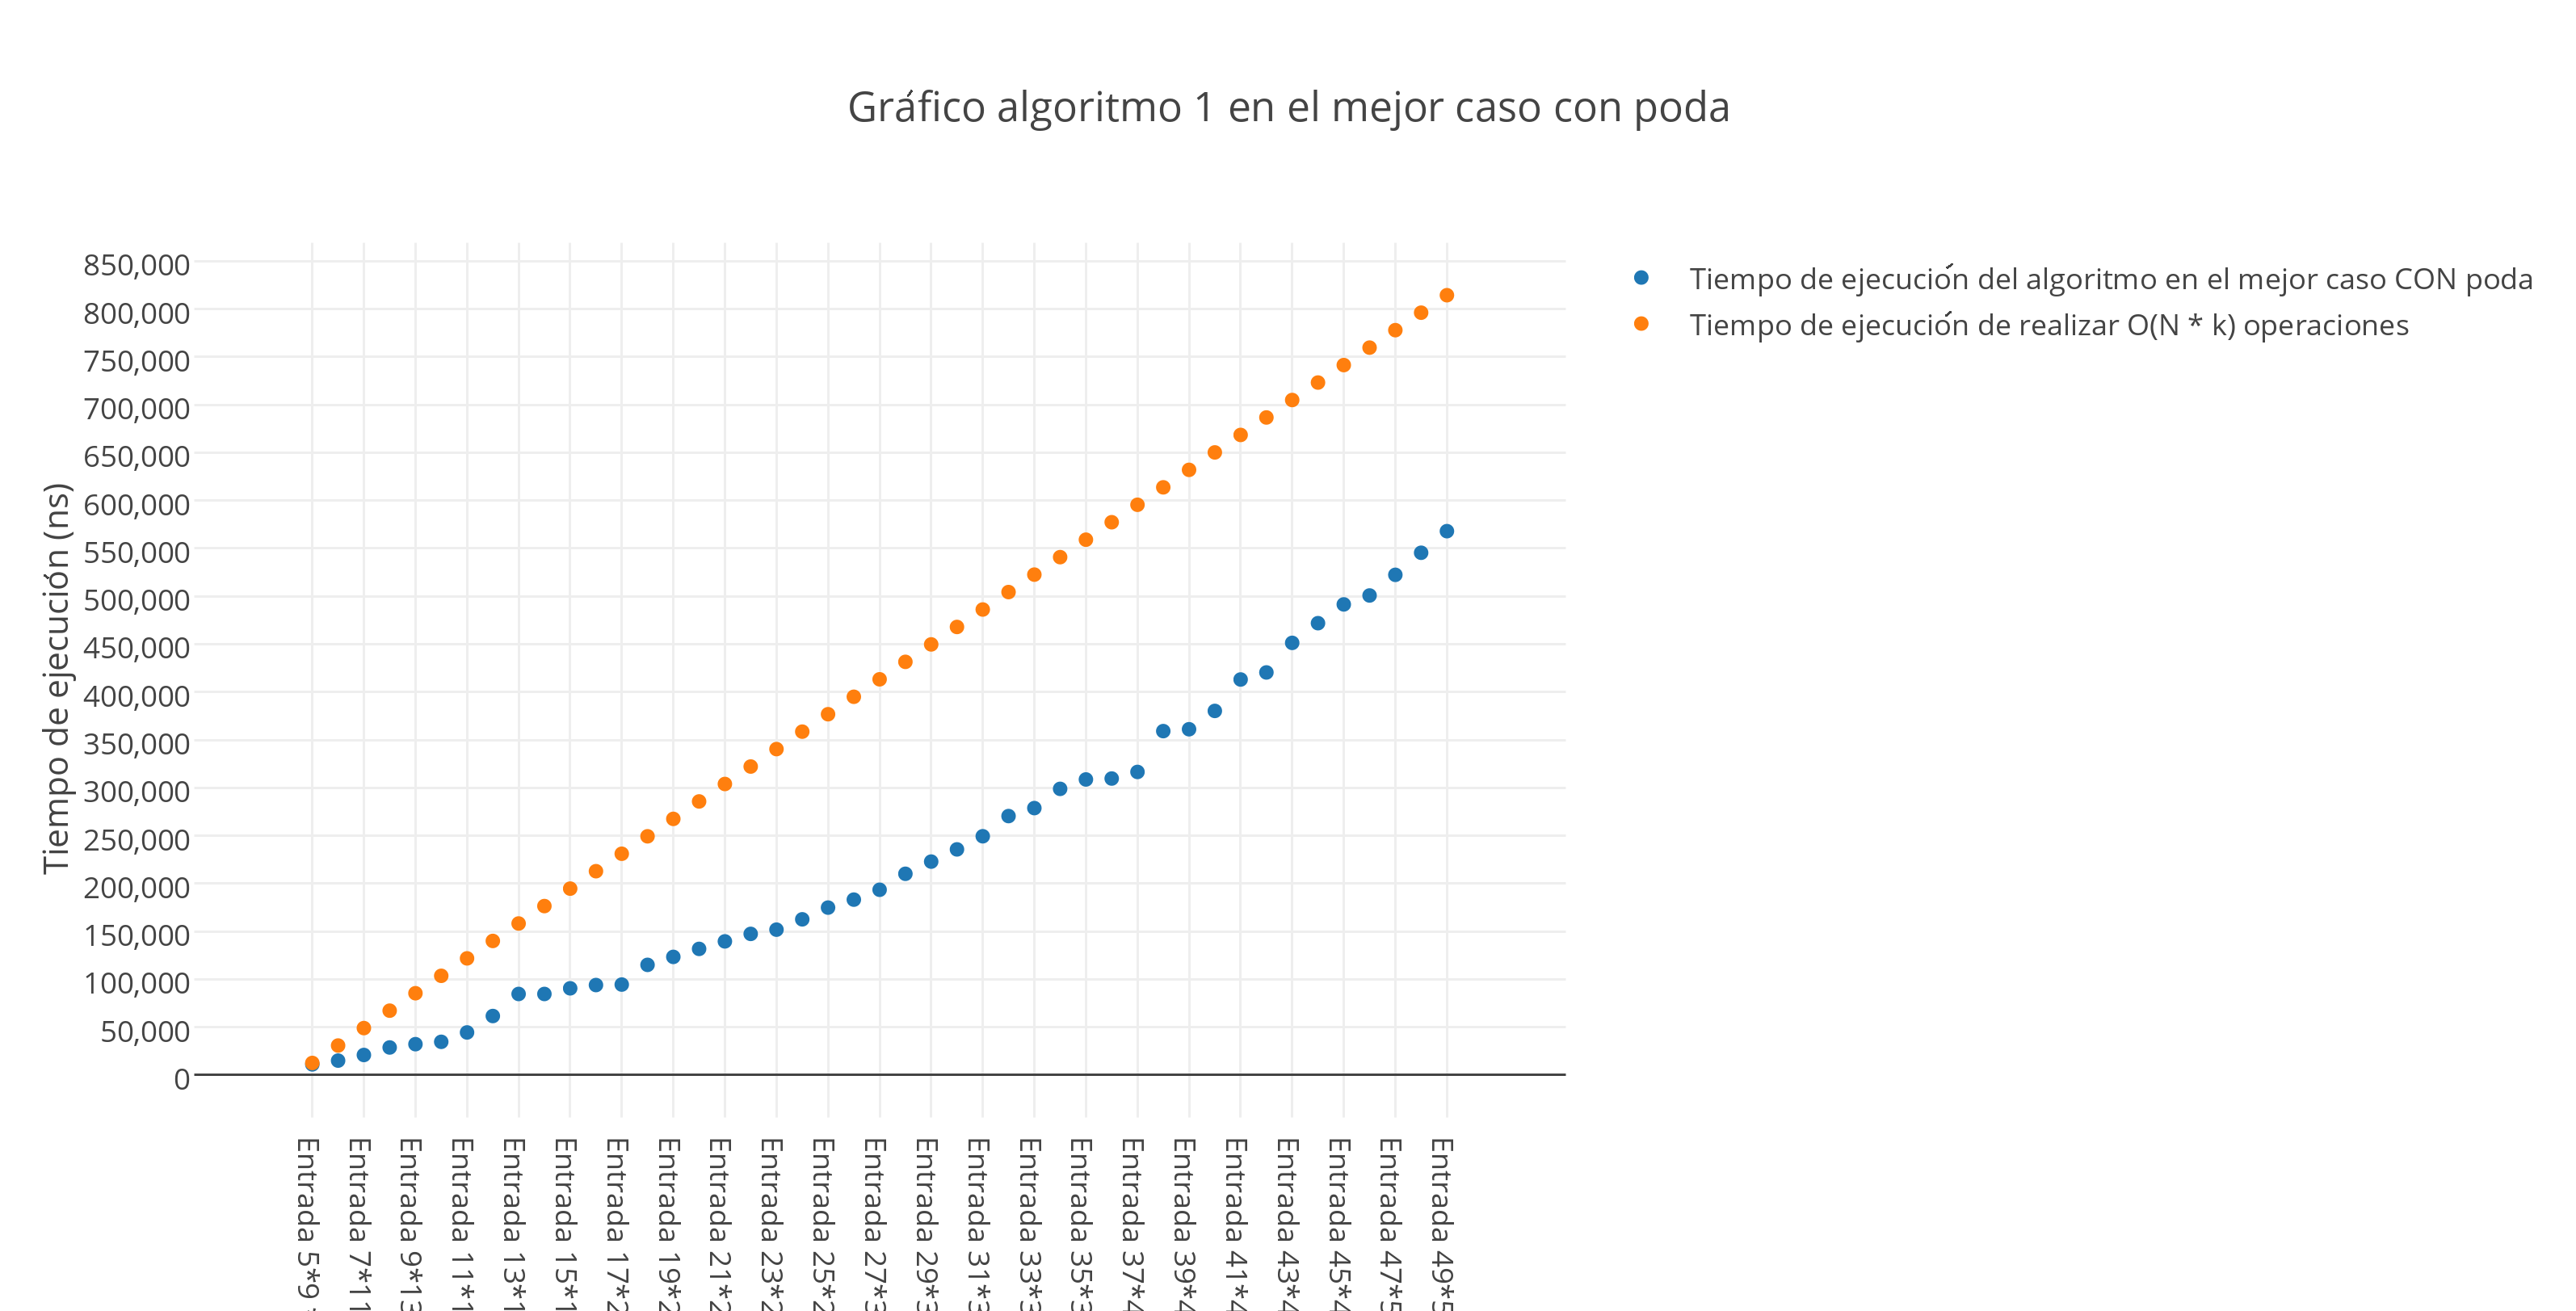
\includegraphics[scale=0.65]{./EJ1/mejorcaso11.png}
 {$Gr$\'a$fico$ \ 1.3 - $Mejor$ $Caso$ $Con$ $Poda$}
  \end{center}
  \vspace*{0.3cm}

 Para obtener dichas instancias nos resulto prudente realizar aproximadamente unas 20 corridas con el mismo input y sacar el promedio de estas 20 corridas para cada instancia para obtener resultados m\'as consisos.\\ 

Se puede observar en la figura 1.1 que a pesar de no realizar la poda enunciada, nos mantenemos dentro de la complejidad anteriormente calculada.\\

Para los casos promedios nuestro algoritmo se comporta de la siguiente forma sin la poda: 

\vspace*{0.3cm} \vspace*{0.3cm}
  \begin{center}
 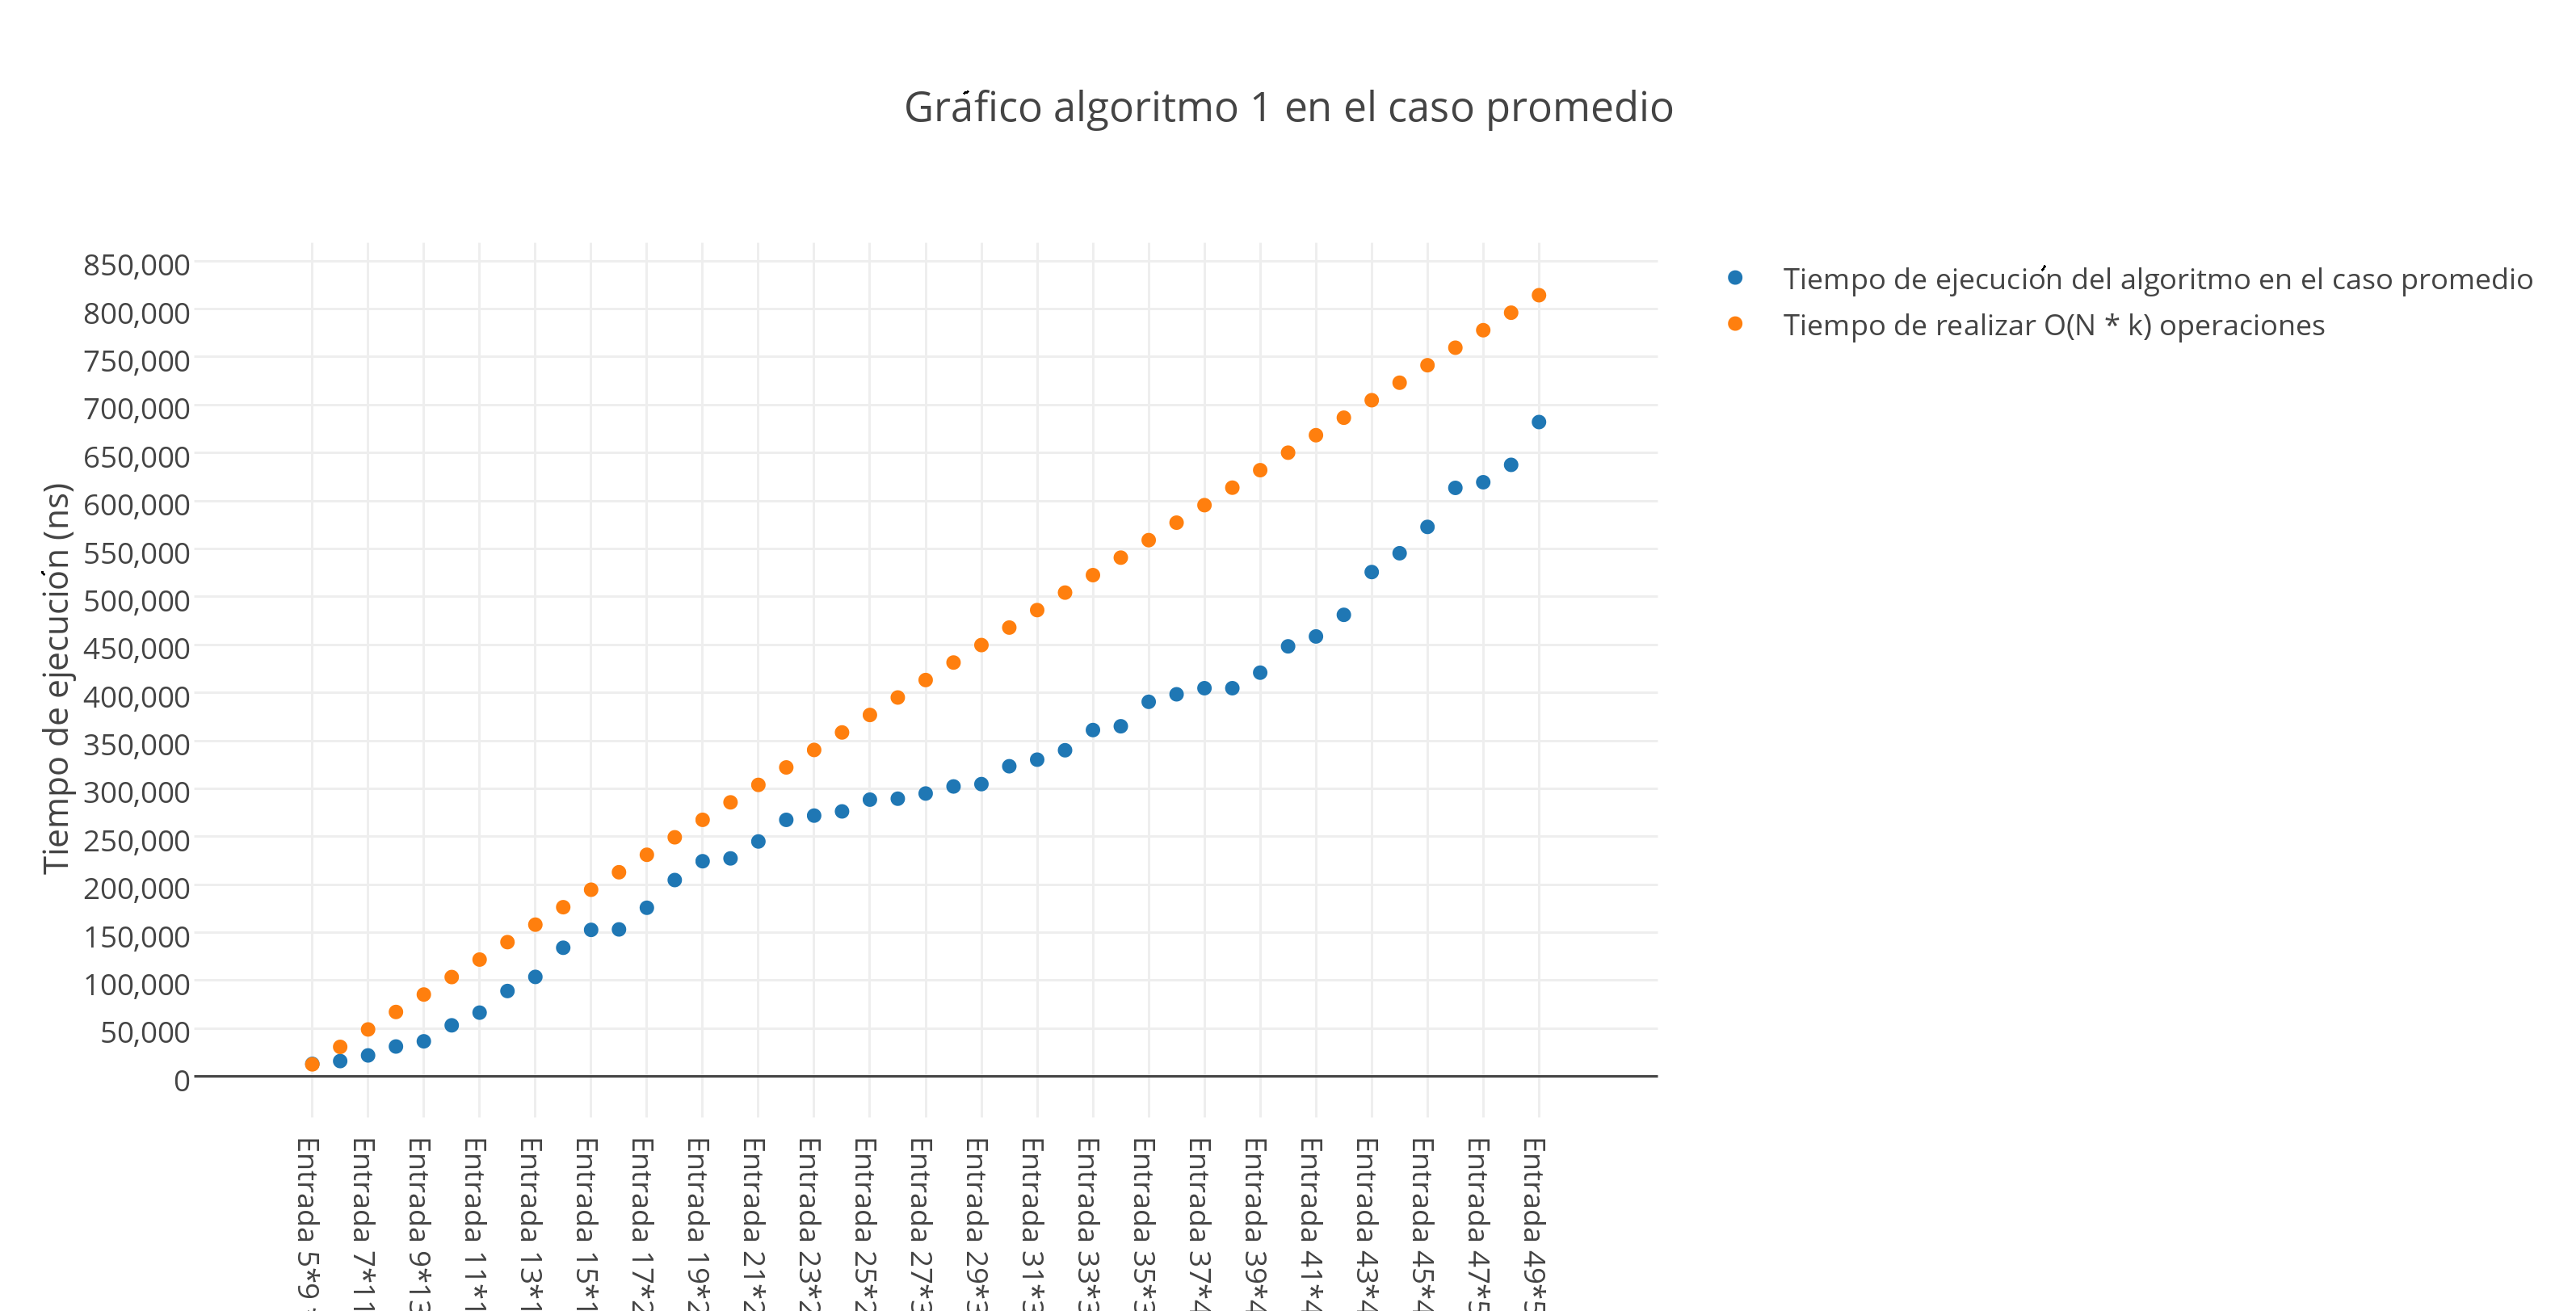
\includegraphics[scale=0.65]{./EJ1/promedio.png}
 {$Gr$\'a$fico$ \ 1.4 - $Caso$ $Promedio$ $Sin$ $Poda$}
  \end{center}
  \vspace*{0.3cm}
  
Y con la poda, la cual puede mejorar para algunos casos dentro de estos promedios el resultado de la comparaci\'on nos arroja lo siguiente:

\vspace*{0.3cm} \vspace*{0.3cm}
  \begin{center}
 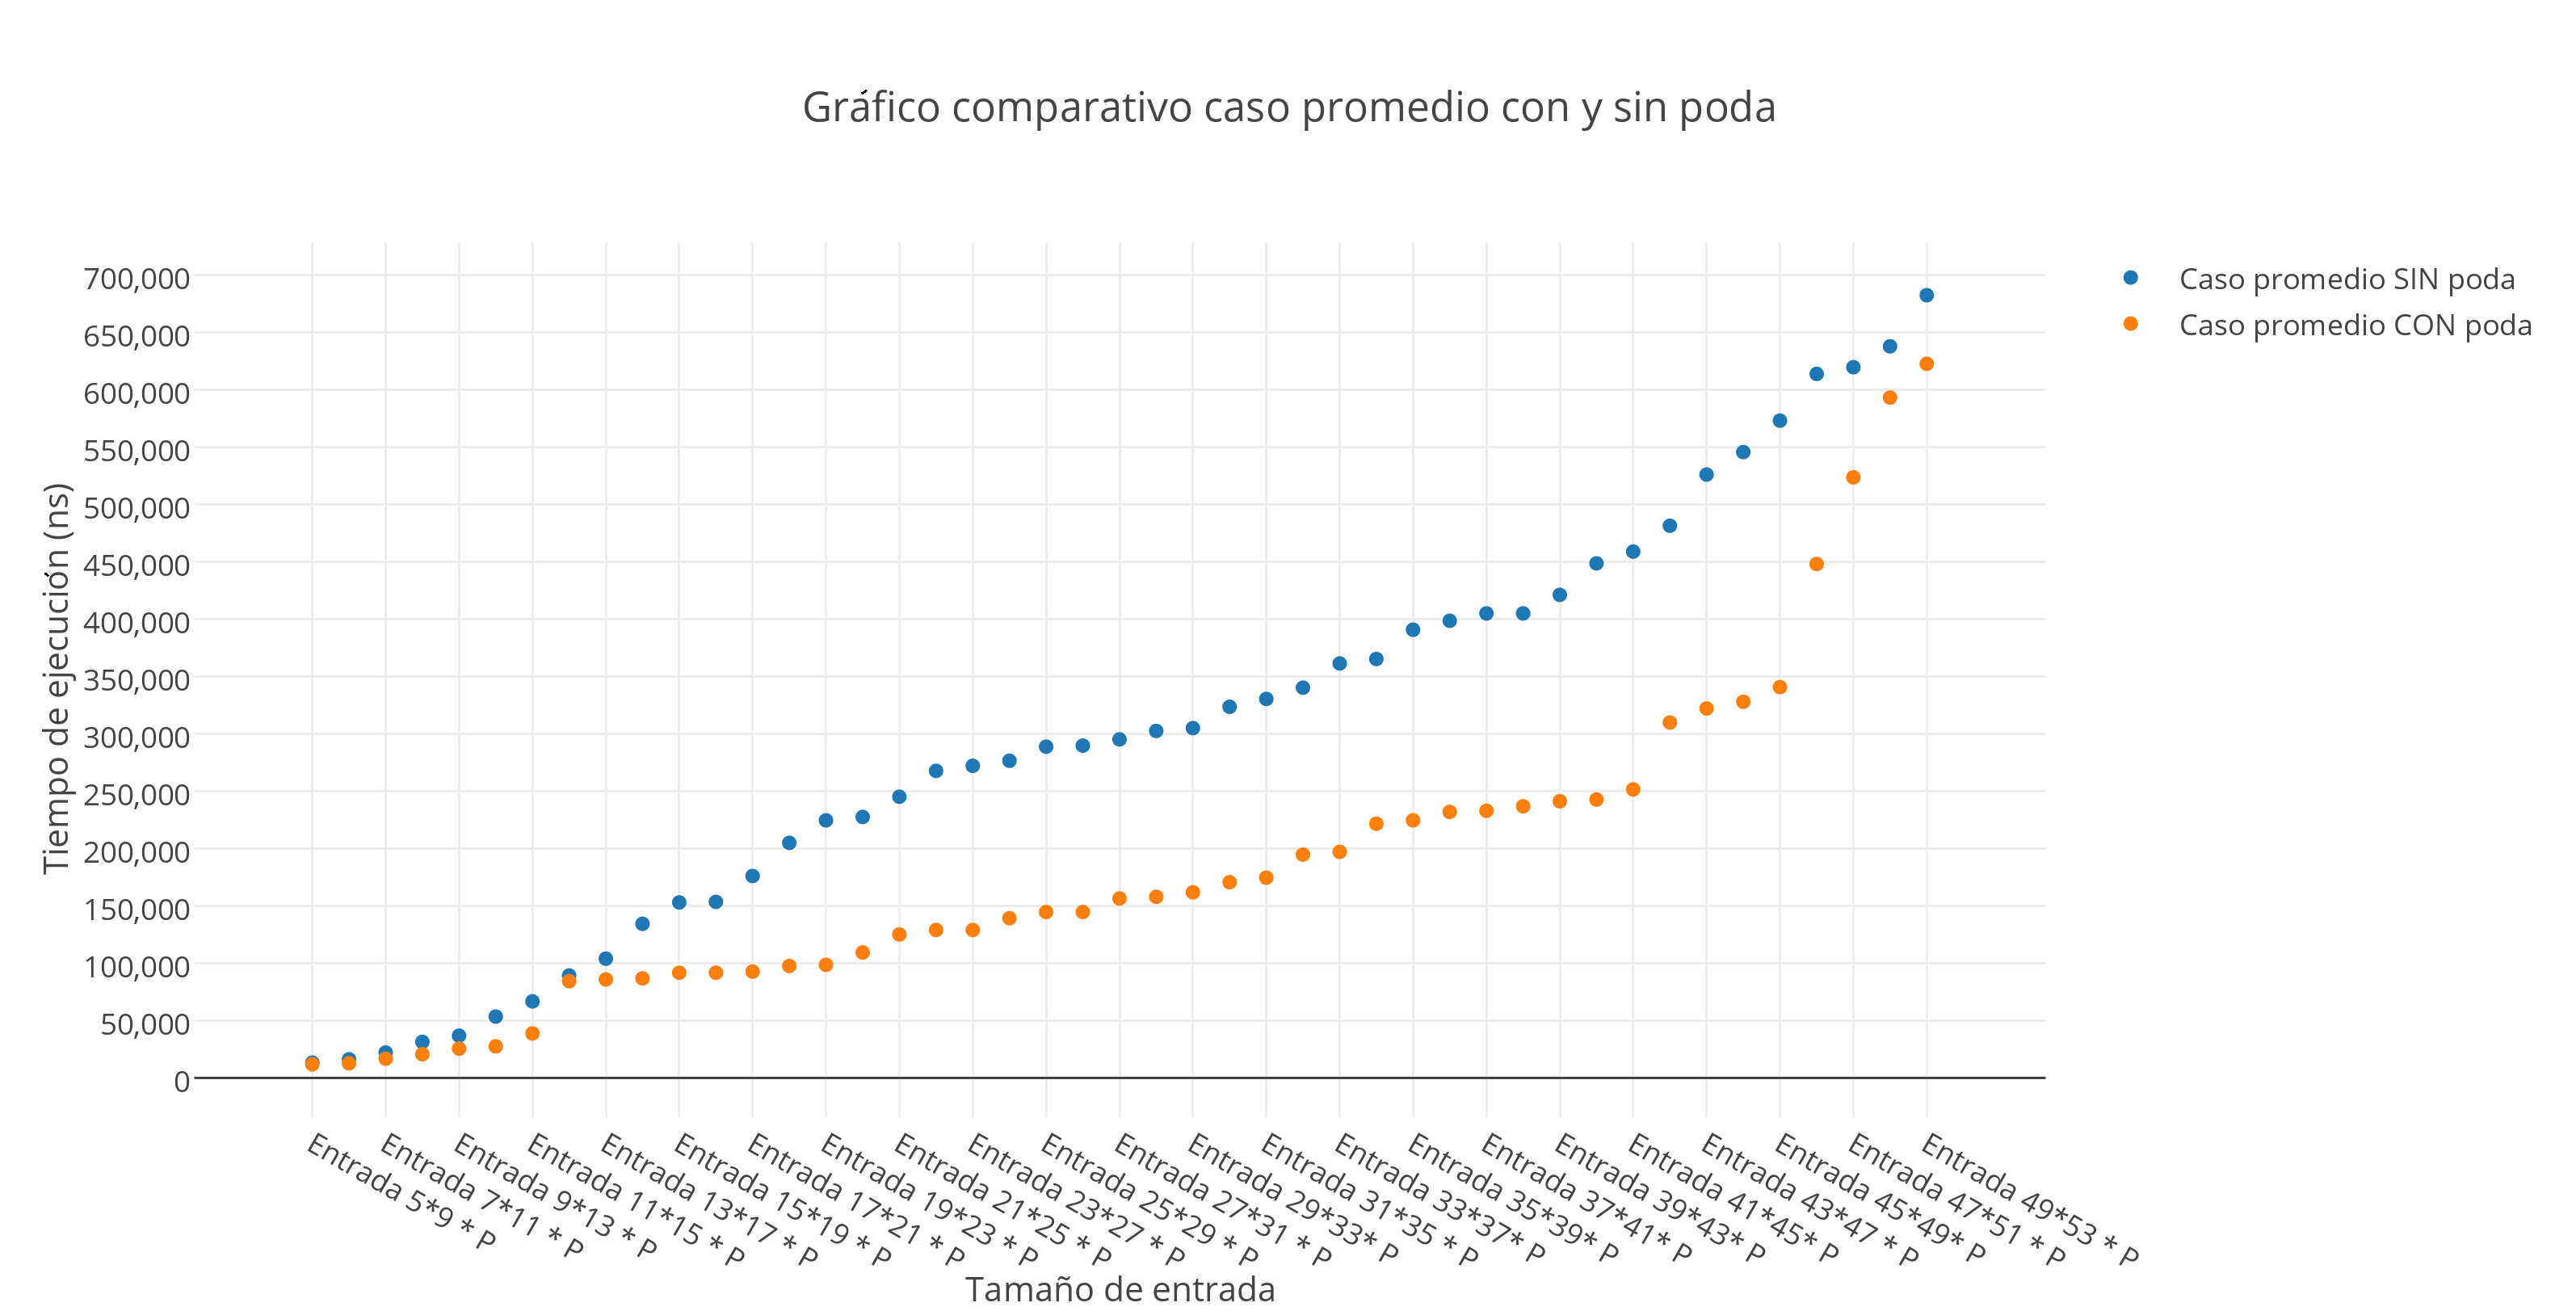
\includegraphics[scale=0.65]{./EJ1/promedio1.png}
 {$Gr$\'a$fico$ \ 1.5 - $Caso$ $Promedio$ $Con$ $y$ $Sin$ $Poda$}
  \end{center}
  \vspace*{0.3cm}
  

\vspace*{0.3cm} \vspace*{0.3cm}
  \begin{center}
 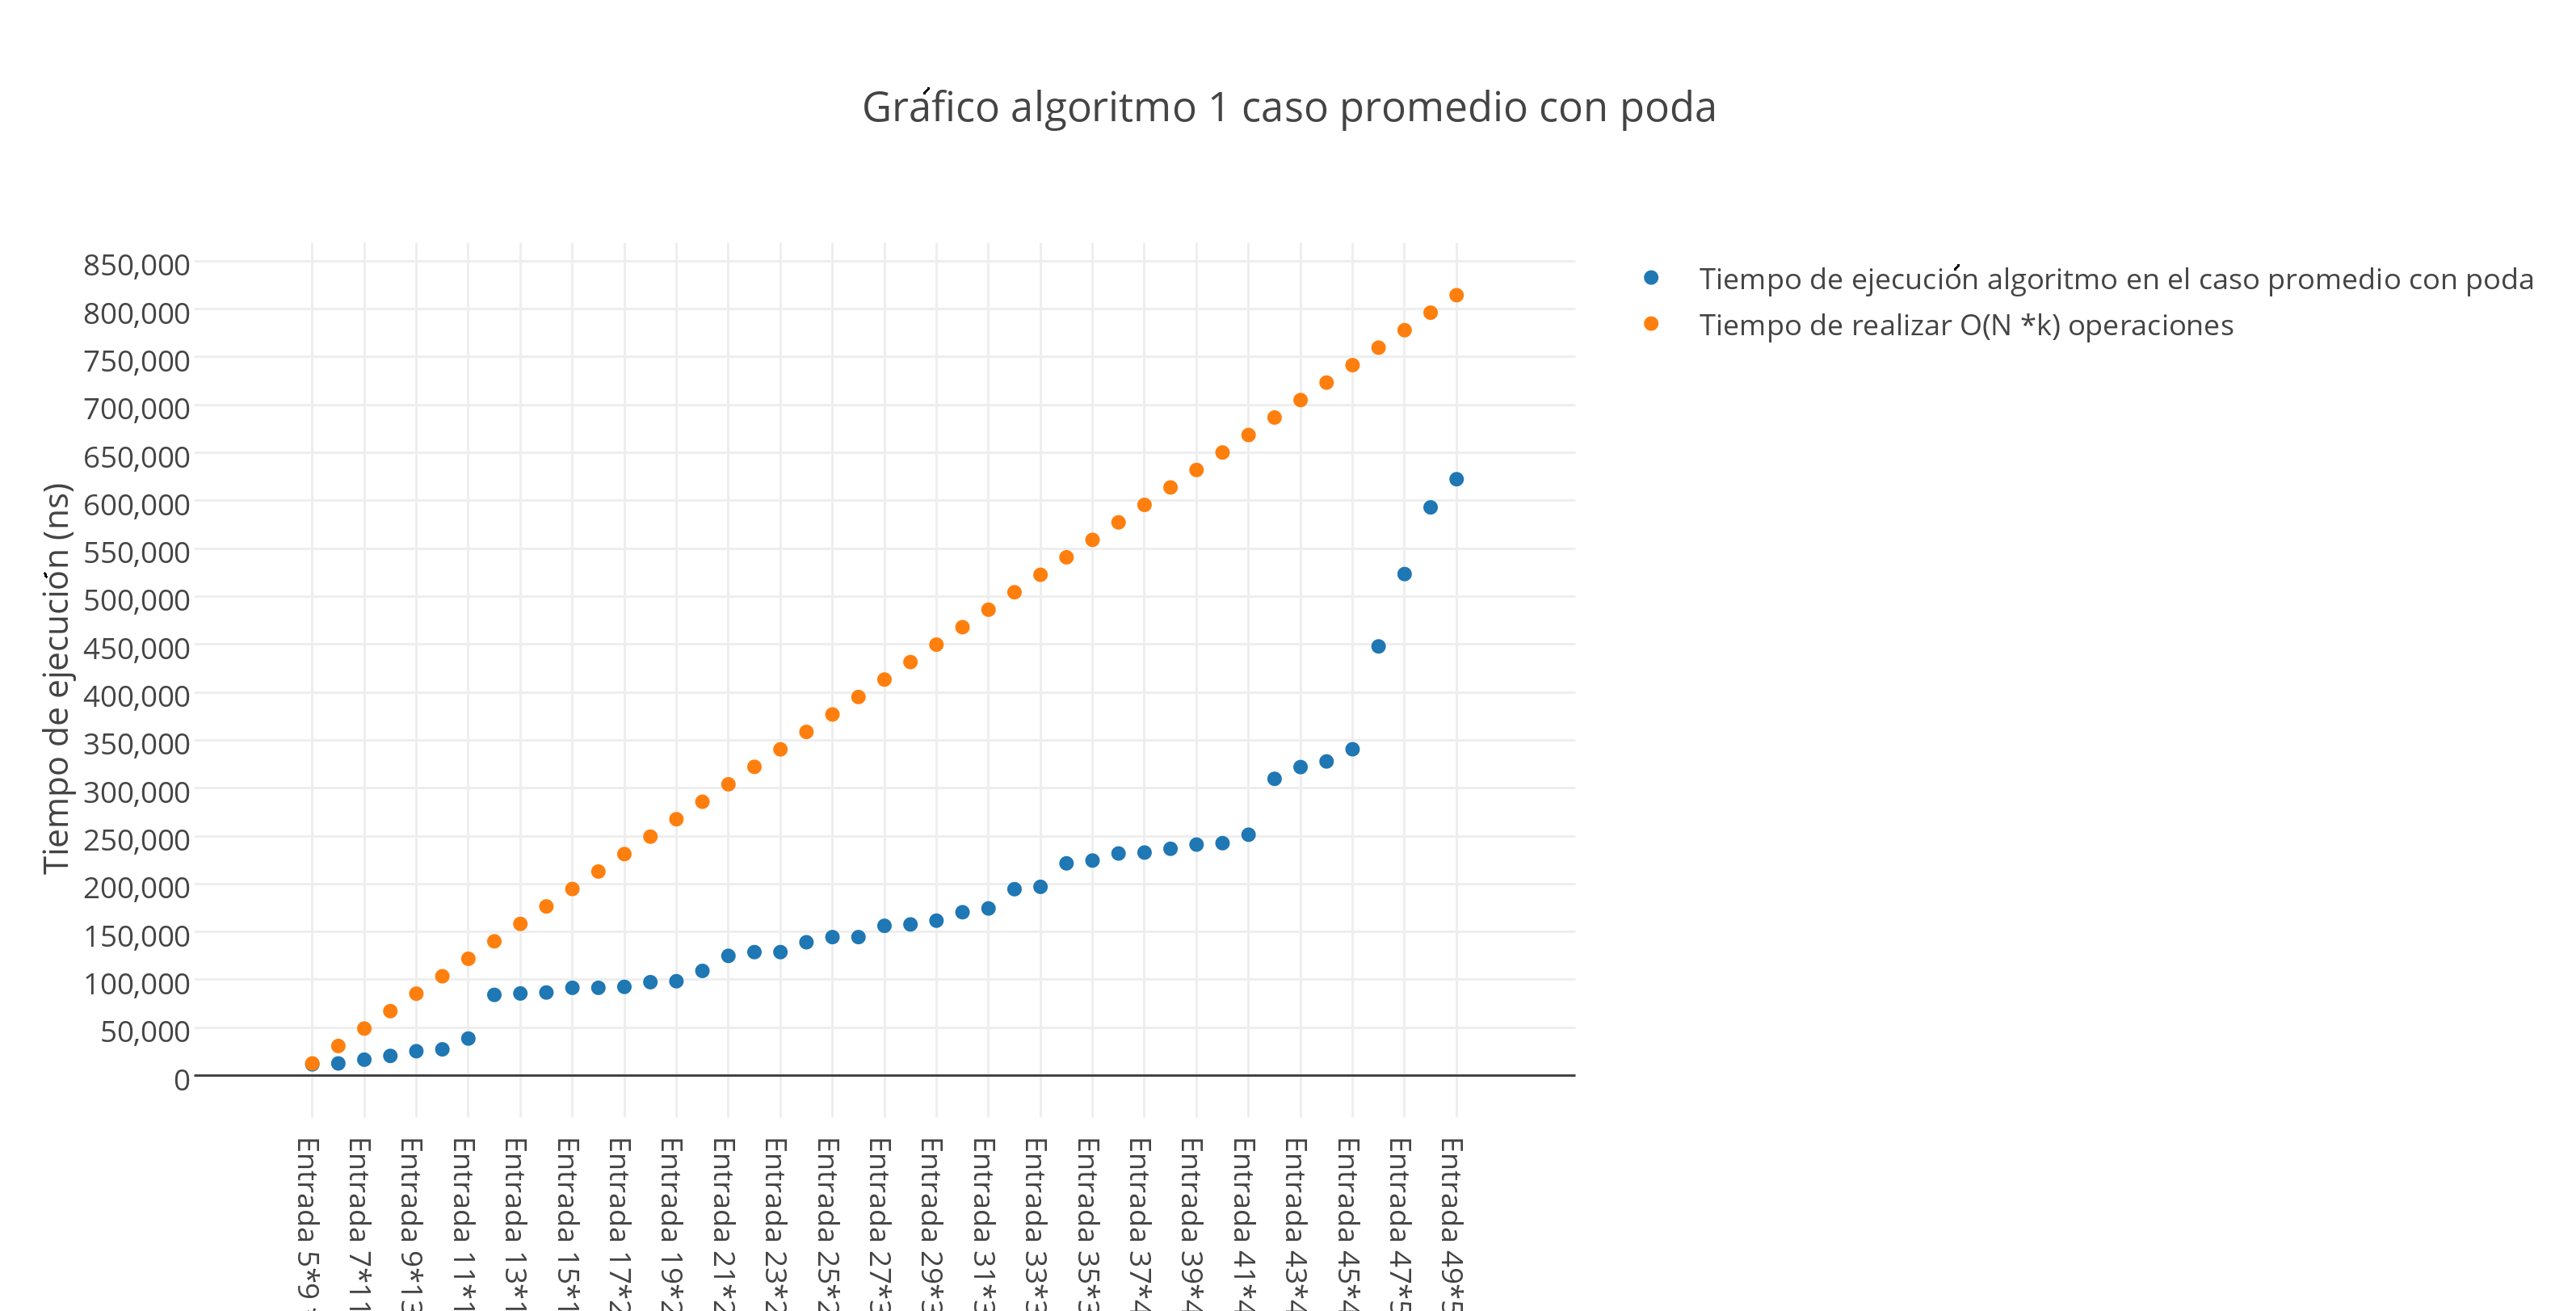
\includegraphics[scale=0.65]{./EJ1/promedio11.png}
 {$Gr$\'a$fico$ \ 1.6 - $Caso$ $Promedio$ $Con$ $Poda$}
  \end{center}
  \vspace*{0.3cm}  
  
  
Se puede observar como el tiempo de ejecuci\'on del "mejor caso" sin poda en el gr\'afico 1.1 es bastante similar al tiempo de ejecuci\'on del caso promedio sin poda (ver gr\'afico 1.4) como hab\'iamos comentado anteriormente.\\

Luego, uno de los peores casos para nuestro algoritmo es en el cual  \textbf{se debe recorrer todos los posibles caminos ya que son todos exactamente iguales}, esto se da as\'i ya que nuestro algoritmo chequea todos los caminos posibles y como todos pueden ser soluci\'on posible avanza por todos y llega al final del laberinto con el mismo valor en todos los posibles caminos\\

\vspace*{0.3cm} \vspace*{0.3cm}
  \begin{center}
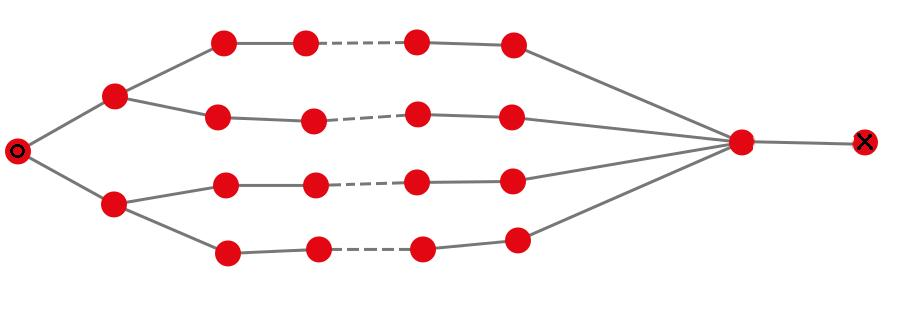
\includegraphics[scale=0.65]{./EJ1/ej1grafopeorcaso.jpeg}
{$Ejemplo Grafo$ \ G1.2 - $Peor$ $Caso$}
  \end{center}
  \vspace*{0.3cm}

Para este grafo realizamos las respectivas mediciones las cuales arrojaron los siguientes resultados:\\


\vspace*{0.3cm} \vspace*{0.3cm}
  \begin{center}
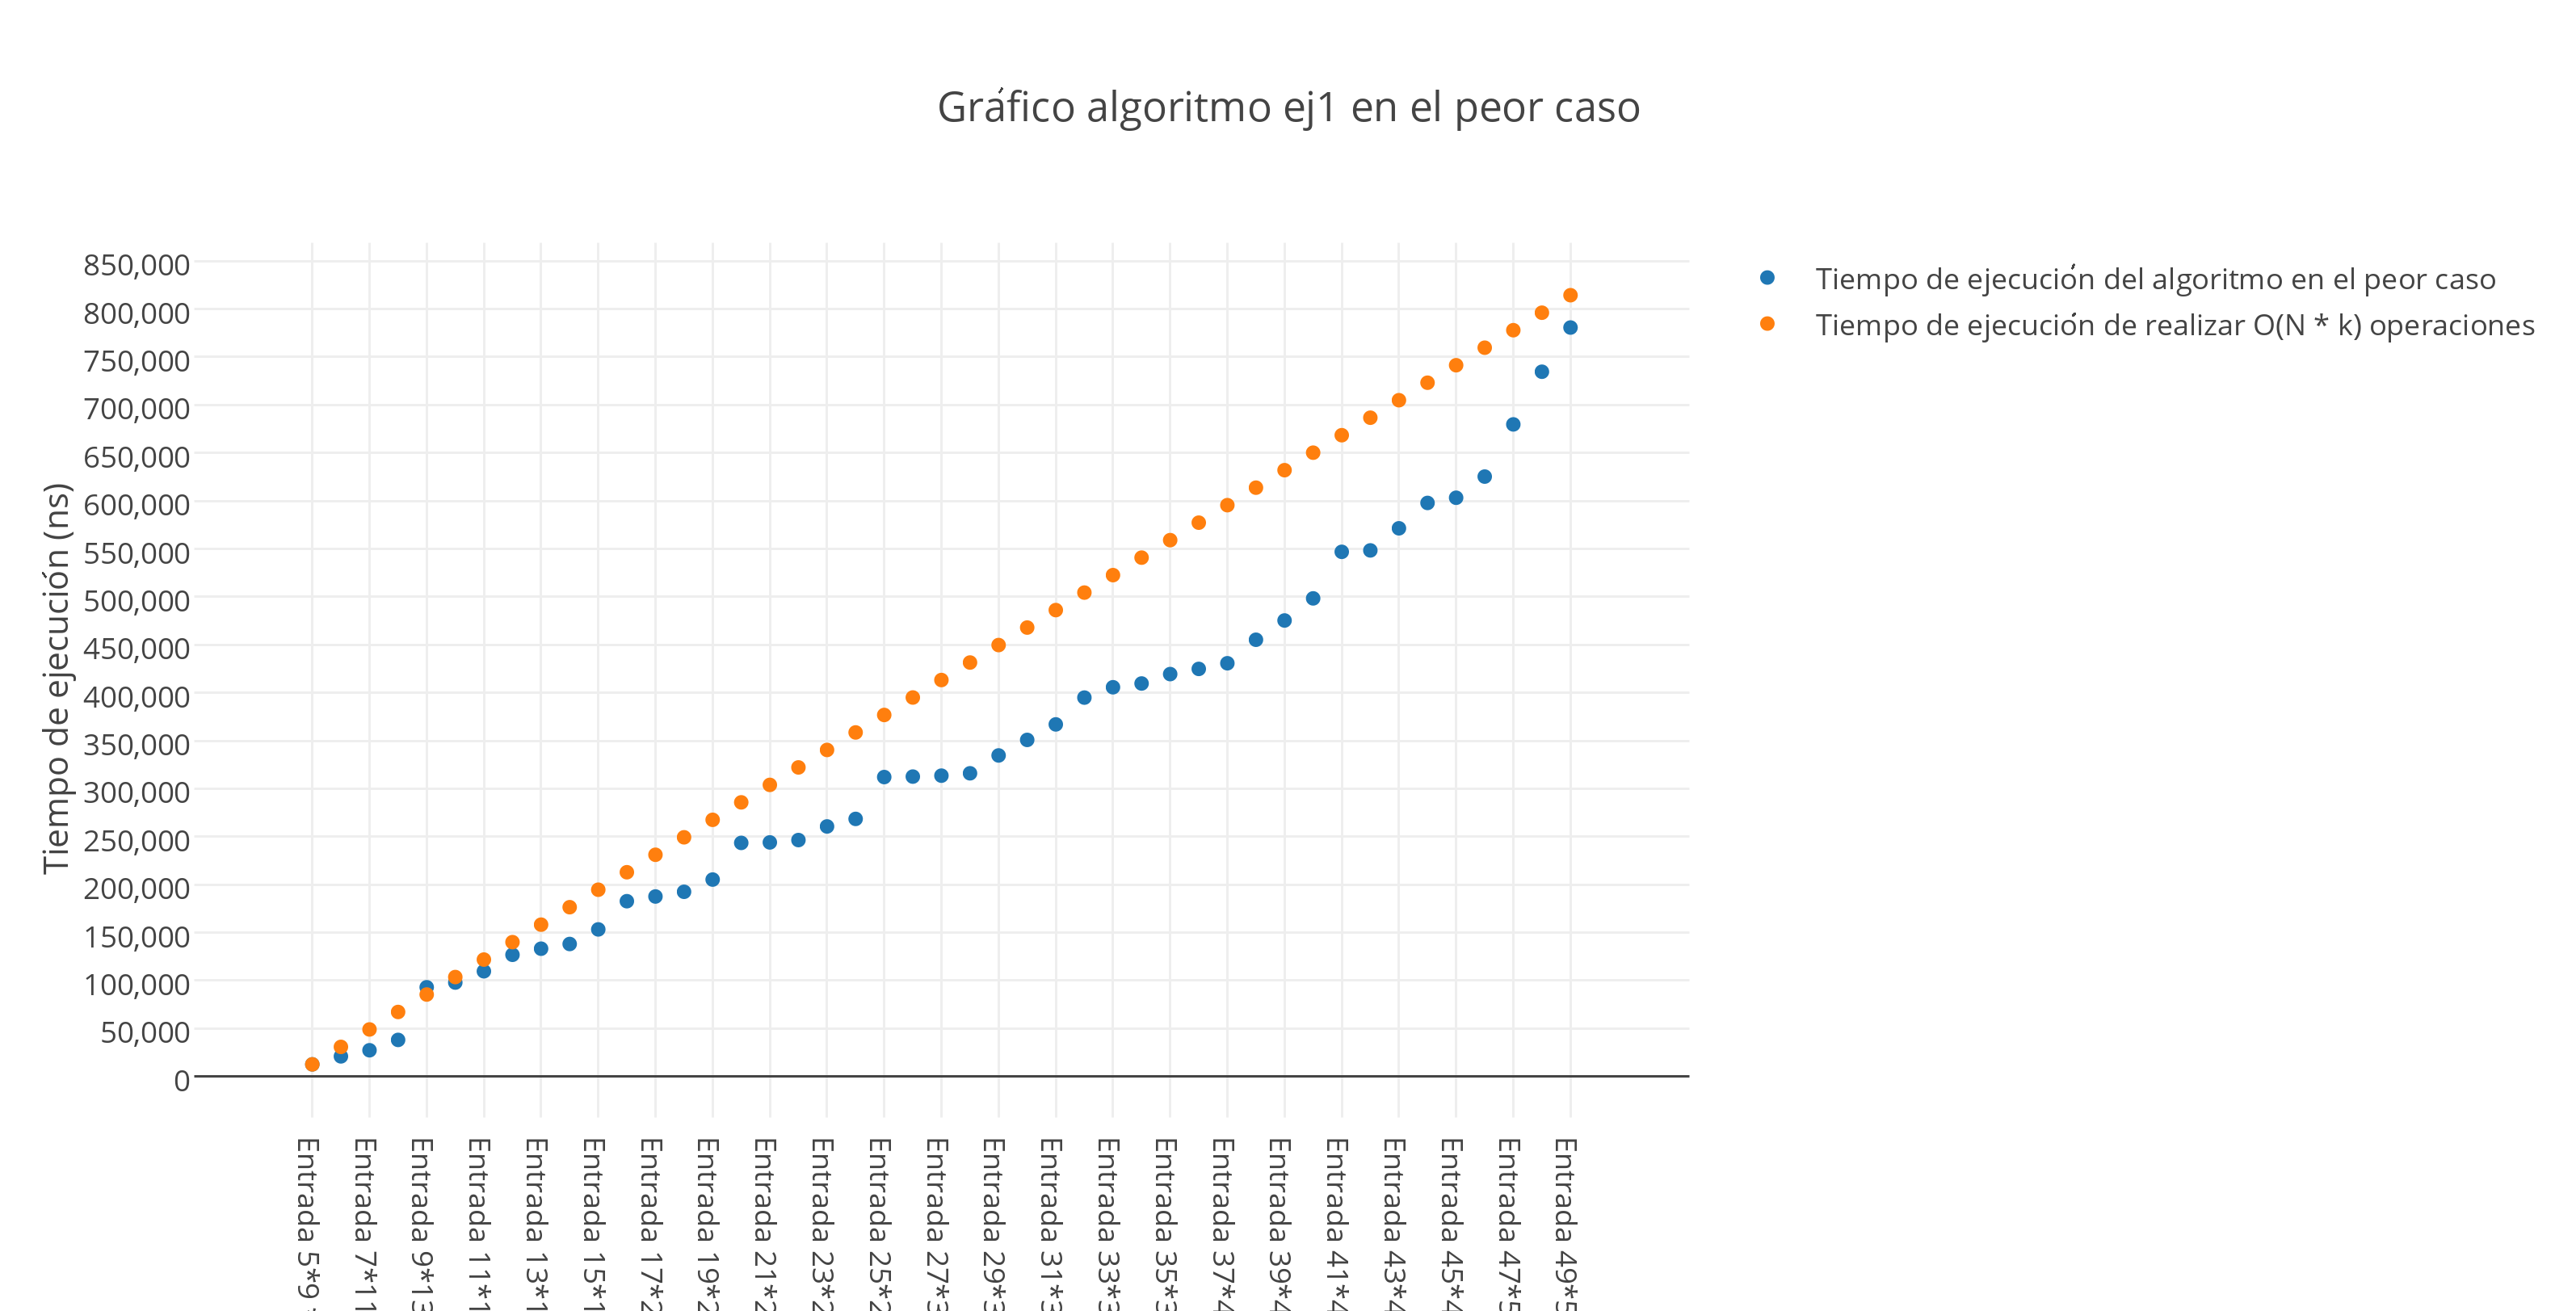
\includegraphics[scale=0.65]{./EJ1/peorcaso.png}
{$Gr$\'a$fico$ \ 1.7 - $Peor$ $Caso$}
  \end{center}
  \vspace*{0.3cm}

Como en el peor caso la poda no sirve ya que hay que recorrer todos los caminos ya que son todos v\'alidos y de igual distancia el tiempo de ejecuci\'on resulta igual

\vspace*{0.3cm} \vspace*{0.3cm}
  \begin{center}
 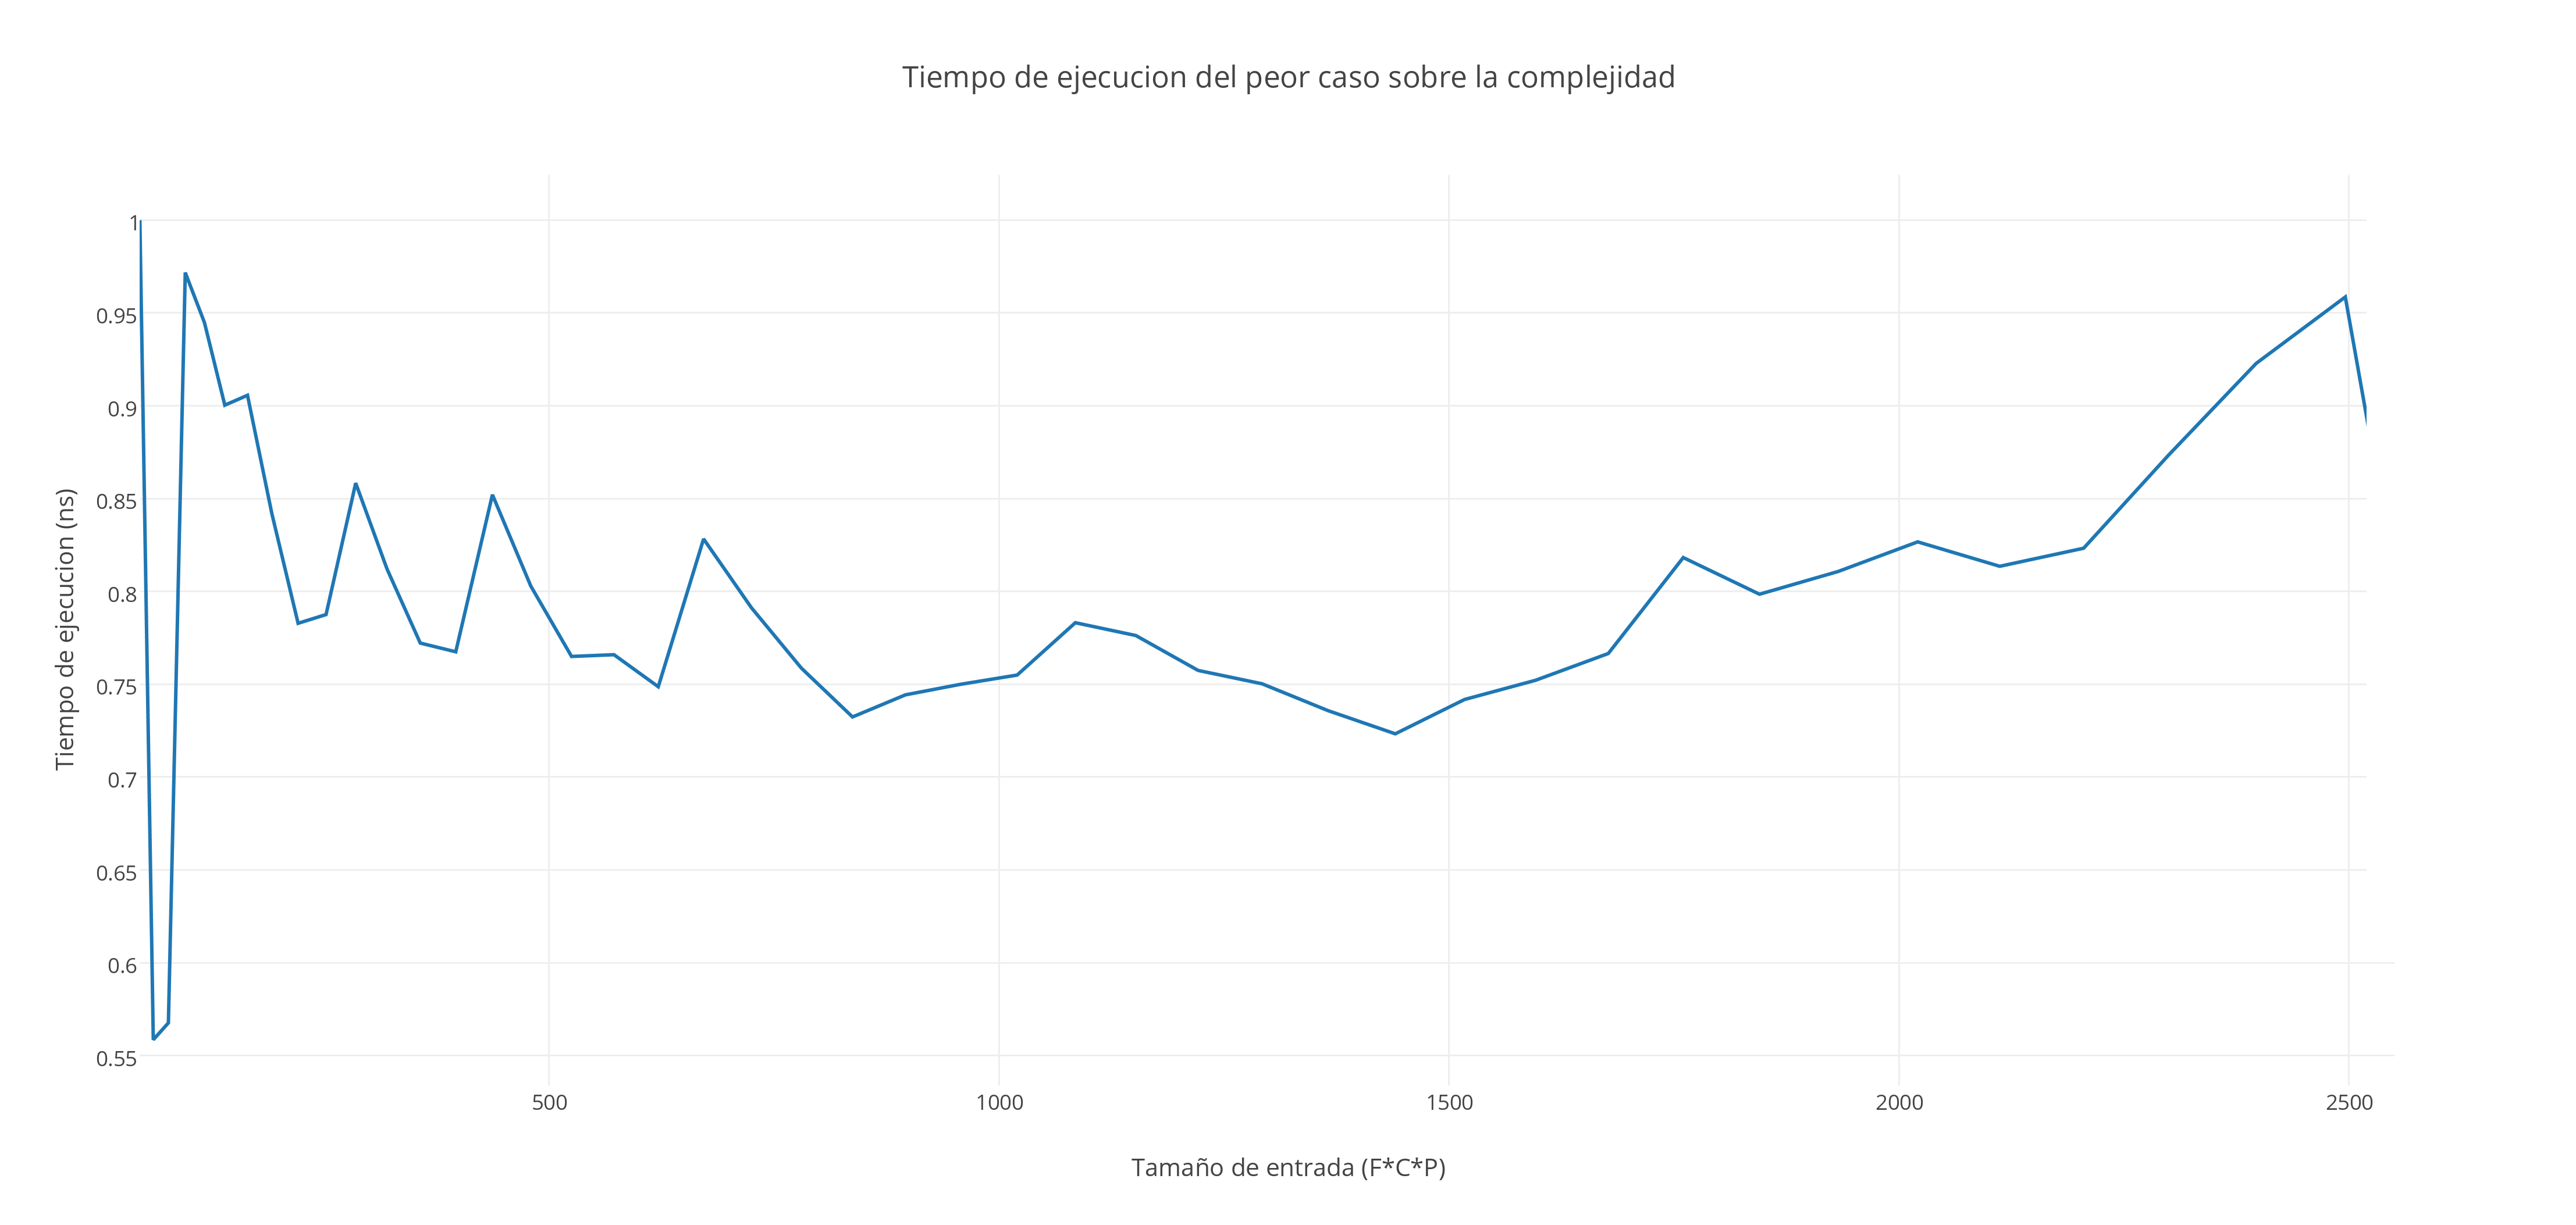
\includegraphics[scale=0.65]{./EJ1/peorcaso1.png}
 {$Gr$\'a$fico$ \ 1.8 - $Peor$ $Caso$ $Con$ $y$ $Sin$ $Poda$}
  \end{center}
   \vspace*{0.3cm}
  
 Para obtener dichas instancias nos resulto prudente realizar aproximadamente unas 20 corridas con el mismo input y sacar el promedio de estas 20 corridas para cada instancia para obtener resultados m\'as consisos.\\ 

Podemos observar en la figura 1.5 como la funci\'on resultante de nuestro algoritmo en el peor caso se mantiene por debajo de la funci\'on final del tiempo de realizar O(N * k) operaciones lo cual fue la complejidad precalculada.\\

Por \'ultimo mostraremos dos gr\'aficos comparativos con el mejor, el peor y el caso promedio sin realizar la poda contra la complejidad precalculada y el segundo mostrar\'a los mismos casos pero con la poda.\\

\vspace*{0.3cm} \vspace*{0.3cm}
  \begin{center}
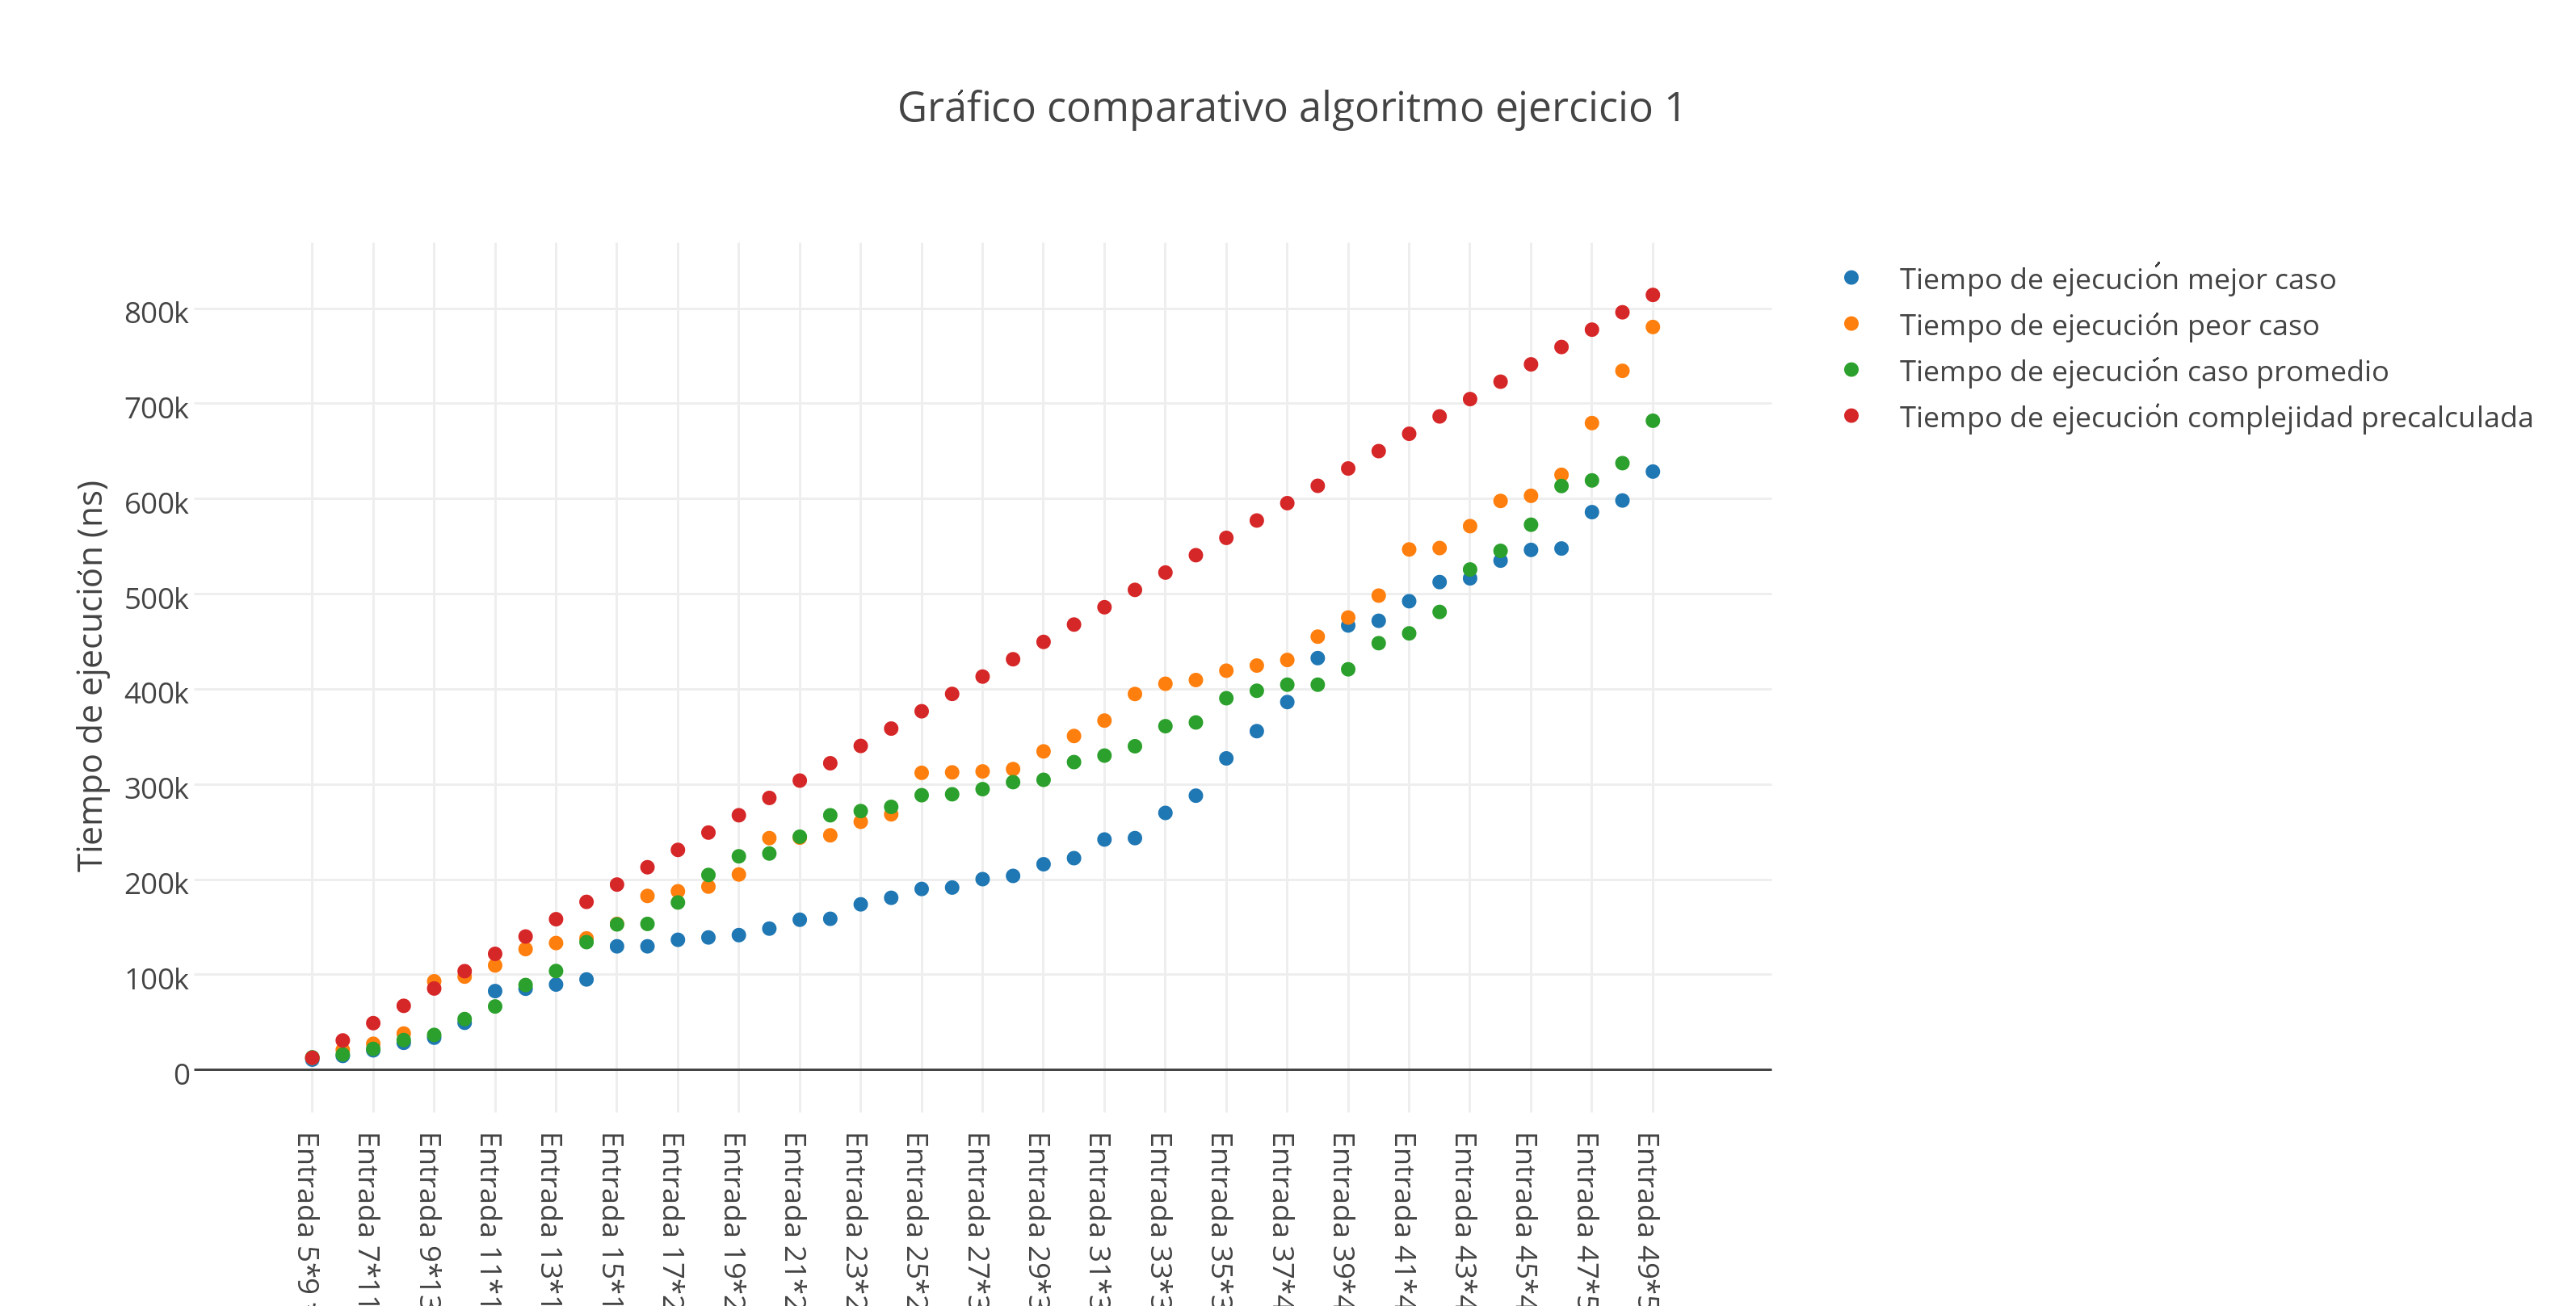
\includegraphics[scale=0.65]{./EJ1/comparativo.png}
{$Gr$\'a$fico$ \ 1.9 - $Comparativo$ $Sin$ $Poda$}
  \end{center}
  \vspace*{0.3cm}
  
  \vspace*{0.3cm} \vspace*{0.3cm}
  \begin{center}
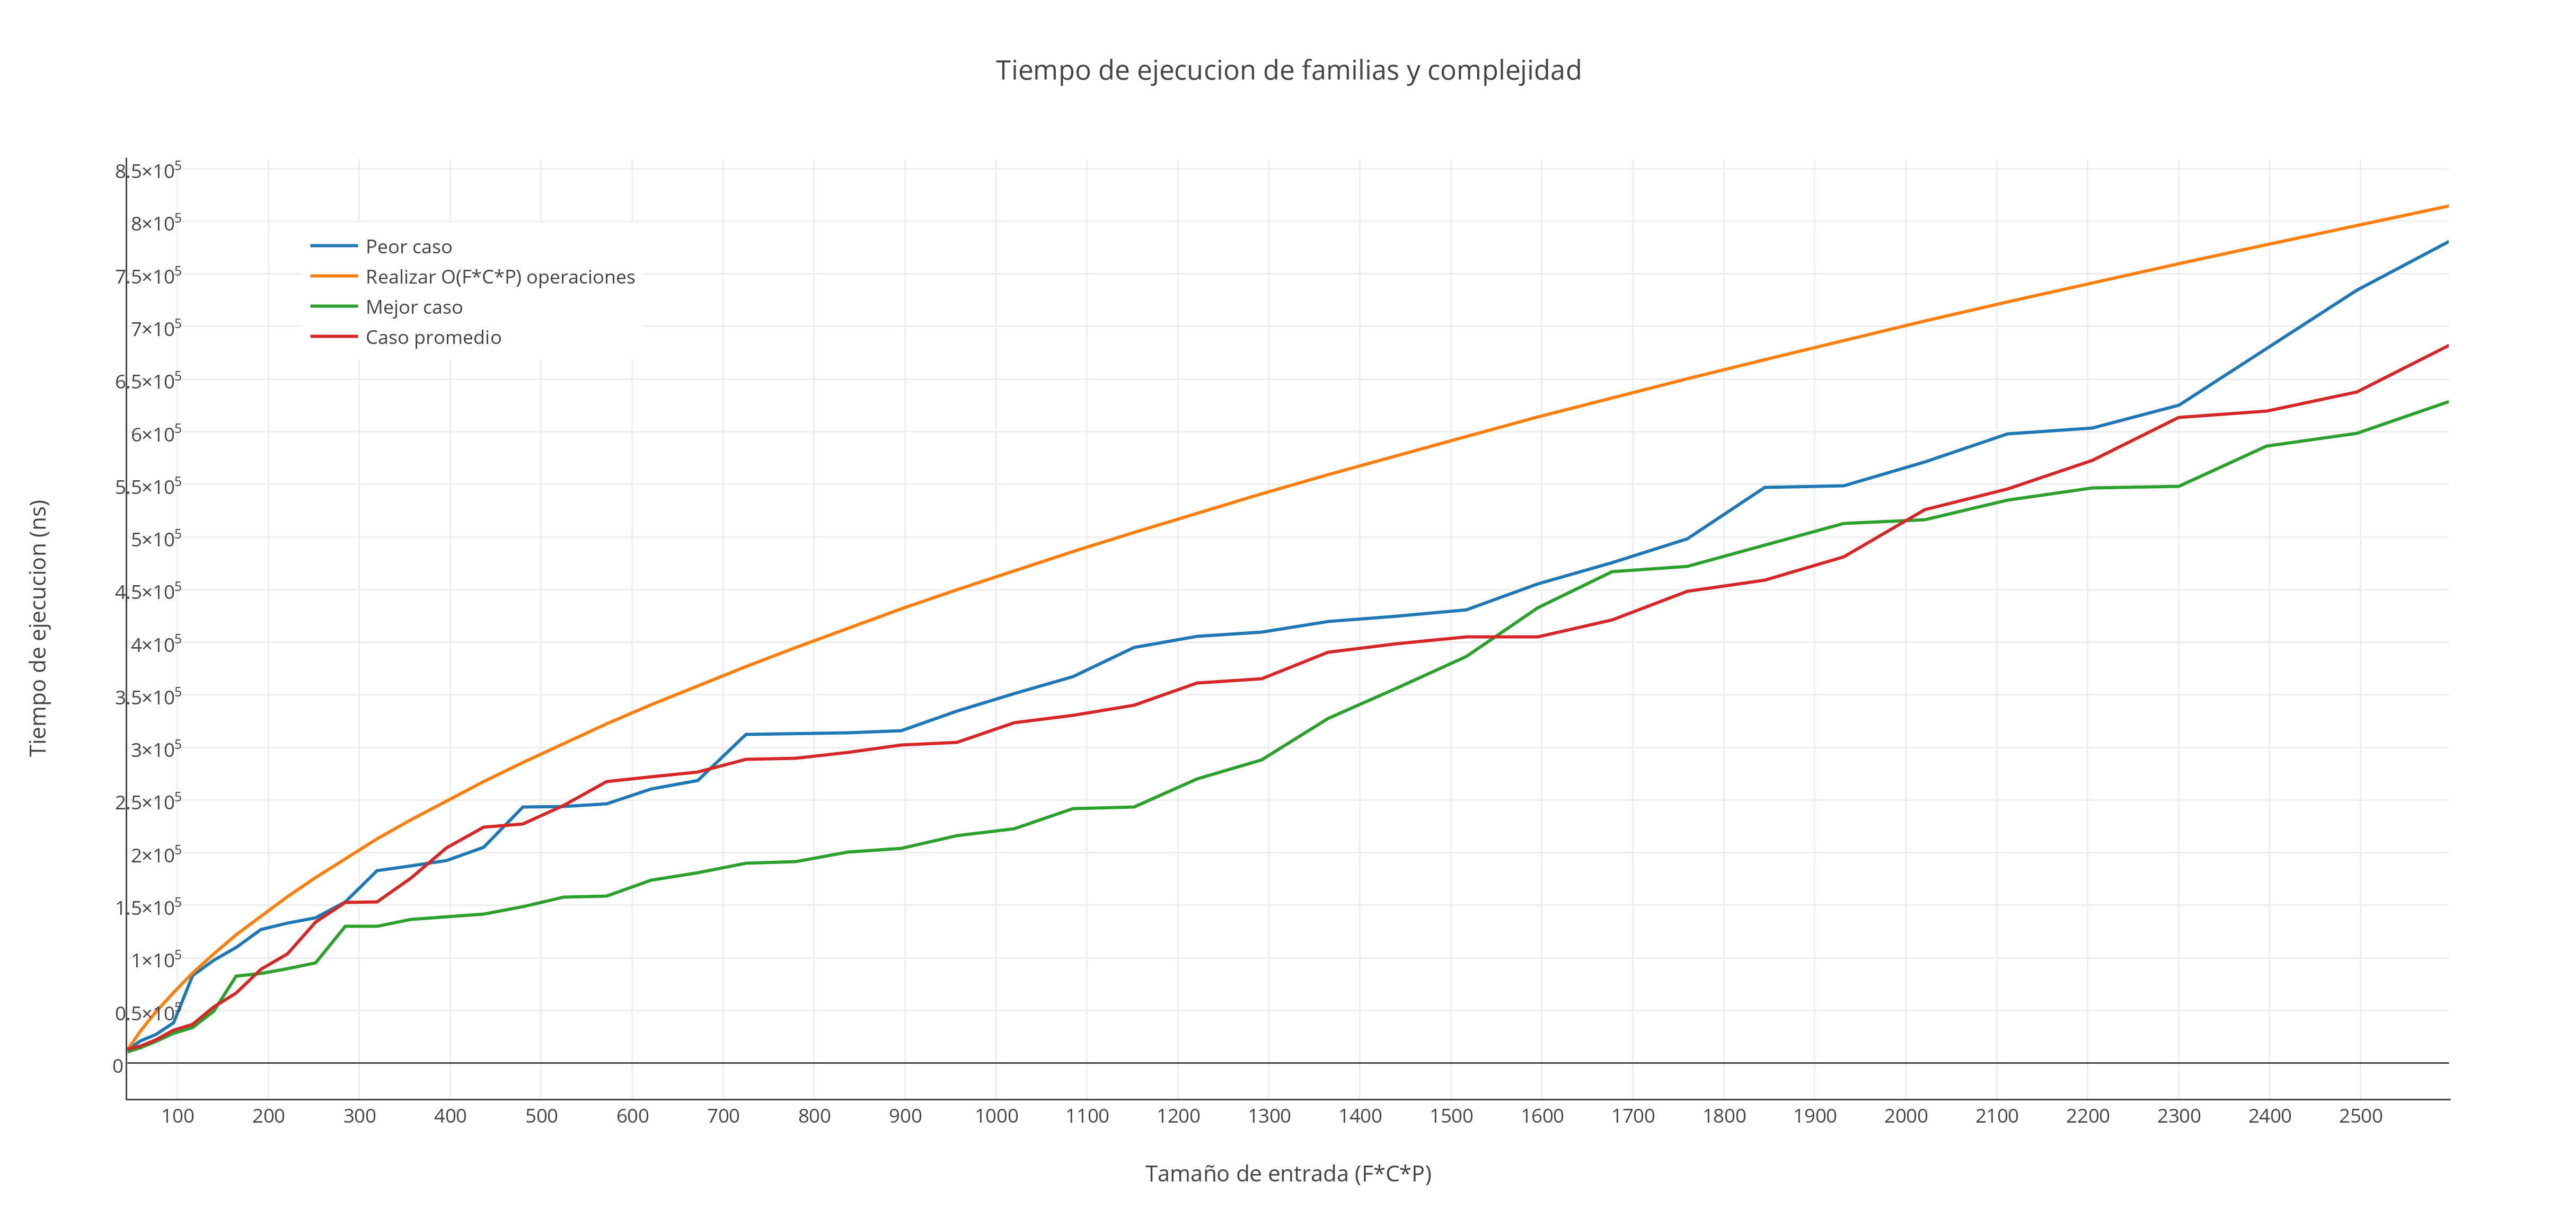
\includegraphics[scale=0.65]{./EJ1/comparativo1.png}
{$Gr$\'a$fico$ \ 1.10 - $Comparativo$ $Con$ $Poda$}
  \end{center}
  \vspace*{0.3cm}


Luego de lo mostrado, podemos ver que ya sea en el peor caso nuestro algoritmo en funci\'on al tiempo de ejecuci\'on queda asintotizado por debajo de la funci\'on del tiempo de la complejidad .